\documentclass[11pt]{article}
\usepackage[margin=1in]{geometry}
\usepackage{booktabs}
\usepackage{graphicx}
\usepackage{amsmath,amssymb}
\usepackage{hyperref}
\usepackage{xcolor}
\usepackage{caption}
\usepackage{subcaption}
\usepackage{array}
\usepackage{multirow}
\usepackage{placeins}

\hypersetup{colorlinks=true, linkcolor=blue, citecolor=blue, urlcolor=blue}

\title{Empirical Analysis of Persuasive Recommendation\\with Endogenous Preference Dynamics:\\[4pt] Evidence from the MIND Dataset}
\author{UBC Gang}
\date{April 2026}

\begin{document}
\maketitle

\begin{abstract}
Do recommendation platforms shape the preferences they claim to serve? We study this question using the Microsoft News Dataset (MIND), which records ${\sim}$1M users' reading behavior over 14 days. A three-period design (baseline taste, intermediate consumption, and future taste) reveals that preferences shift toward what users click, not toward what they see. Cosine similarity between user taste and article features predicts clicks well (MNL AUC $= 0.707$), validating an inner-product utility specification. Taste shifts toward consumption with a permutation $z$-score of 515, and session-level self-reinforcement averages $+243\%$ across all 14 content categories. Click-through rate decays $3.4\times$ from the nearest to the farthest articles, yielding a persuasion radius of $d \leq 0.66$ that feed position cannot extend. Distant clicks produce larger taste shifts than nearby ones ($r = 0.528$), creating a tension between what is likely to be clicked and what moves taste.

The sharpest finding concerns the role of engagement. Categories shown but not clicked shift taste \emph{away} from those categories, below the baseline of never having been shown at all (within-user Cohen's $d = -0.75$, 13 of 14 categories). The backfire intensifies with the dose of ignored exposure ($\rho = -0.21$). (This might be relevant to fatigue or Berlyne’s two-factor theory, nut we need to discuss in a meeting.) Clicked content, by contrast, reliably reinforces taste, is self-accelerating with no satiation, and partially persists after overshoot. These findings ground the core assumptions of a theoretical model of persuasive recommendation and characterize the fine structure (self-acceleration, mean-reversion, and category asymmetry) that any optimization must accommodate.
\end{abstract}


%======================================================================
\section{Data and Design}
%======================================================================

\subsection{Datasets}

We use both versions of the Microsoft News Dataset (Table~\ref{tab:datasets}).

\begin{table}[ht]
\centering
\caption{MIND dataset summary. Each impression contains a user's click history and a list of shown articles with binary click labels.}
\label{tab:datasets}
\begin{tabular}{llccc}
\toprule
Dataset & Split & Dates & Impressions & Users \\
\midrule
\multirow{2}{*}{MINDsmall} & Train & Nov 9--14 & 156,965 & \multirow{2}{*}{94,057} \\
 & Dev & Nov 15 & 73,152 & \\
\midrule
\multirow{3}{*}{MINDlarge} & Train & Nov 9--14 & 2,232,748 & \multirow{3}{*}{${\sim}$1M} \\
 & Dev & Nov 15 & 376,471 & \\
 & Test & Nov 16--22 & 2,370,727 & \\
\bottomrule
\end{tabular}
\end{table}
\FloatBarrier

Each impression contains the user's accumulated click history and a list of articles shown with binary click labels. The test set lacks labels but retains click histories, enabling P3 click inference via history growth. Each article belongs to one of 15 categories and 285 subcategories. Total unique articles: 104,151 (large), 51,282 (small).

\subsection{Notation and representations}
\label{sec:notation}

Let $i$ index users and $j$ index articles. Each article $j$ has a feature vector $\mathbf{v}_j$ and belongs to one of the 15 MIND categories: news, sports, finance, lifestyle, health, travel, foodanddrink, autos, entertainment, video, weather, tv, movies, music, and kids.

We use two article embeddings for $\mathbf{v}_j$: a subcategory one-hot vector ($\mathbb{R}^{285}$) with full coverage, and the average of pre-trained Wikidata entity embeddings ($\mathbb{R}^{100}$) with 73.7\% coverage. User $i$'s taste vector $\boldsymbol{\theta}_i$ is the mean embedding of their clicked articles.

For category-level analyses, we represent each user's taste as a distribution $\boldsymbol{\theta}_i \in \mathbb{R}^{14}$, where $\theta_{i,k}$ is user $i$'s click fraction in category~$k$. The kids category is excluded from this vector because it has insufficient observations (fewer than 100 clicks across the dataset); the remaining 14 categories account for over 99.9\% of all clicks. In the substitution analysis (Section~\ref{sec:assortment}), all 15 categories are retained because that test operates at the impression level rather than requiring a user-level taste vector.

\subsection{Three-period design}
\label{sec:three_period_design}

The 14-day MINDlarge window supports a three-period design. Period~1 (P1, Nov 9--11) captures baseline taste. Period~2 (P2, Nov 12--15) captures intermediate consumption and exposure. Period~3 (P3, Nov 16--22) captures future taste, inferred from test-set history growth. Throughout, $\boldsymbol{\theta}_i^{(\text{P}t)}$ denotes user $i$'s taste vector in period $t$.

\subsection{Analysis sample}

Sections~\ref{sec:utility}--\ref{sec:assortment} use 50,000 sampled users (187,088 impressions, 7.15M article-level observations). The three-period taste analysis samples 100,000 users for session-level tests and uses the full design on 143,574 users with $\geq 2$ clicks in each period. The exposure analysis uses 145,985 users with $\geq 2$ clicks in P1 and P2, $\geq 5$ shown articles in P2, and $\geq 2$ inferred P3 clicks. The base click rate is 4.07\%.


%======================================================================
\section{Inner-Product Utility}
\label{sec:utility}
%======================================================================

The theoretical model assumes that user $i$'s utility for article $j$ is the inner product $u_{ij} = \langle \boldsymbol{\theta}_i, \mathbf{v}_j \rangle$, where $\boldsymbol{\theta}_i$ is the user's taste vector and $\mathbf{v}_j$ is the article's feature vector (both defined in Section~\ref{sec:notation}). If correct, cosine similarity should predict the click-through rate (CTR), defined as the fraction of shown articles that the user clicks.

We compute $\text{sim}_{ij} = \cos(\boldsymbol{\theta}_i, \mathbf{v}_j)$ for each (user, article) pair and bin by quintile. Table~\ref{tab:sim_quintile} reports the results.

\begin{table}[ht]
\centering
\caption{CTR by cosine-similarity quintile. Higher similarity between user taste and article features predicts higher click-through rates.}
\label{tab:sim_quintile}
\begin{tabular}{cccc}
\toprule
Sim quintile & Mean similarity & CTR & $N$ \\
\midrule
0 (lowest) & 0.000 & 2.86\% & 4,290,400 \\
1 & 0.070 & 4.18\% & 715,294 \\
2 & 0.163 & 4.94\% & 715,077 \\
3 & 0.298 & 5.95\% & 715,185 \\
4 (highest) & 0.587 & 8.49\% & 714,526 \\
\bottomrule
\end{tabular}
\end{table}
\FloatBarrier

CTR nearly triples from the lowest to the highest quintile. To quantify this relationship continuously, we compute the point-biserial correlation between $\text{sim}_{ij}$ and the binary click indicator (1 if user $i$ clicked article $j$, 0 otherwise). This correlation measures the linear association between a continuous variable (similarity) and a binary outcome (click). Using subcategory embeddings, $r = 0.095$ ($p < 10^{-300}$); using entity embeddings, $r = 0.055$ ($p < 10^{-300}$). Both are modest in magnitude but overwhelmingly significant given the sample size, confirming that articles more similar to a user's taste are more likely to be clicked.

A multinomial logit (MNL) sharpens the test. For an impression showing articles $j = 1, \ldots, J$, the probability that user $i$ clicks article $j$ is $P(\text{click } j) = \exp(\beta \cdot \text{sim}_{ij}) / \sum_{k=1}^{J} \exp(\beta \cdot \text{sim}_{ik})$, where $\beta$ is estimated by maximum likelihood. Table~\ref{tab:auc} reports AUC on 100,000 held-out impressions.

\begin{table}[ht]
\centering
\caption{Click prediction accuracy (AUC) by predictor. The MNL uses only category-level similarity as input.}
\label{tab:auc}
\begin{tabular}{lc}
\toprule
Predictor & AUC \\
\midrule
Subcategory cosine similarity & 0.613 \\
Entity cosine similarity & 0.576 \\
Combined & 0.618 \\
MNL (subcategory features only) & \textbf{0.707} \\
\bottomrule
\end{tabular}
\end{table}
\FloatBarrier

An AUC of 0.707 using only category-level features (no article text, recency, or position) validates the inner-product specification. The controlled regression in Section~\ref{sec:regression} reinforces this: historical taste predicts clicks with $\beta = 0.39$ ($R^2 = 0.41$) after controlling for the assortment. Taste is a genuine latent state, not an artifact of what the algorithm shows.


%======================================================================
\section{Taste Dynamics}
\label{sec:taste}
%======================================================================

\subsection{Self-reinforcement}

A single click in a category more than triples the probability of returning to it in the next session. For each category, we compare $P(\text{click in session } t{+}1 \mid \text{clicked in session } t)$ to $P(\text{click in session } t{+}1 \mid \text{not clicked in session } t)$. The lift is the percentage increase: $(\,P_{\text{click}} - P_{\text{no click}}\,) / P_{\text{no click}}$. Table~\ref{tab:selfreinforcement} reports the results for all 14 categories.

\begin{table}[ht]
\centering
\caption{Session-level self-reinforcement by category. Lift measures the percentage increase in next-session click probability after clicking a category versus not clicking it.}
\label{tab:selfreinforcement}
\small
\begin{tabular}{lcccr}
\toprule
Category & $P(\text{next} \mid \text{click})$ & $P(\text{next} \mid \text{no click})$ & Lift & $p$-value \\
\midrule
autos & 0.127 & 0.023 & $+448\%$ & $< 10^{-300}$ \\
video & 0.068 & 0.019 & $+254\%$ & $< 10^{-300}$ \\
foodanddrink & 0.118 & 0.036 & $+232\%$ & $< 10^{-300}$ \\
weather & 0.061 & 0.024 & $+154\%$ & $< 10^{-143}$ \\
health & 0.080 & 0.034 & $+132\%$ & $< 10^{-300}$ \\
travel & 0.058 & 0.026 & $+127\%$ & $< 10^{-234}$ \\
entertainment & 0.077 & 0.035 & $+122\%$ & $< 10^{-300}$ \\
movies & 0.031 & 0.014 & $+123\%$ & $< 10^{-71}$ \\
sports & 0.243 & 0.113 & $+114\%$ & $< 10^{-300}$ \\
lifestyle & 0.193 & 0.105 & $+84\%$ & $< 10^{-300}$ \\
tv & 0.068 & 0.044 & $+53\%$ & $< 10^{-129}$ \\
finance & 0.116 & 0.080 & $+45\%$ & $< 10^{-184}$ \\
news & 0.353 & 0.245 & $+44\%$ & $< 10^{-300}$ \\
music & 0.077 & 0.060 & $+29\%$ & $< 10^{-54}$ \\
\midrule
\textbf{Overall} & \textbf{0.184} & \textbf{0.054} & $\boldsymbol{+243\%}$ & $< 10^{-300}$ \\
\bottomrule
\end{tabular}
\end{table}
\FloatBarrier

All 14 categories are significant ($p < 10^{-54}$ or better), replicating on MINDsmall ($+242\%$). The overall lift of $+243\%$ means that a user who clicked a category in one session is $3.4\times$ more likely to click it again in the next session than a user who did not. Niche categories produce the strongest reinforcement (autos: $+448\%$, video: $+254\%$) because their low base rate ($P(\text{next} \mid \text{no click}) \approx 2\%$) leaves more room for a proportional jump. Broad categories reinforce in absolute terms but show smaller lifts (news: $+44\%$, music: $+29\%$) because their base rates are already high. The pattern is consistent with a model in which each click updates the user's taste vector toward the clicked category, with the update being proportionally larger when the category was previously underrepresented.

\subsection{Three-period taste shift}
\label{sec:three_period}

Using the three-period design defined in Section~\ref{sec:three_period_design}, we define the taste shift as $\Delta\boldsymbol{\theta}_i = \boldsymbol{\theta}_i^{(\text{P3})} - \boldsymbol{\theta}_i^{(\text{P1})}$ and test whether its direction aligns with intermediate consumption. For each user, we compute the cosine similarity between the taste shift and three consumption vectors: P1 consumption alone (a placebo), P2 consumption alone, and pooled P1+P2 consumption. A positive cosine means taste moved \emph{toward} what the user consumed; zero means no directional relationship. Table~\ref{tab:taste_alignment} reports the results for 143,574 users with $\geq 2$ clicks in each period.

\begin{table}[ht]
\centering
\caption{Cosine alignment between taste shift and consumption direction. P3 taste shift aligns strongly with P2 consumption.}
\label{tab:taste_alignment}
\begin{tabular}{lccc}
\toprule
Test & Mean $\cos$ & $t$-stat & $p$-value \\
\midrule
$\cos(\text{P2 shift}, \text{P1 consumption})$ & $-0.008$ & $-8.1$ & $4 \times 10^{-16}$ \\
$\cos(\text{P3 shift}, \text{P2 consumption})$ & $\boldsymbol{+0.360}$ & $\boldsymbol{429}$ & $\boldsymbol{< 10^{-300}}$ \\
$\cos(\text{P3 shift}, \text{P1{+}P2 consumption})$ & $+0.397$ & $501$ & $< 10^{-300}$ \\
\bottomrule
\end{tabular}
\end{table}
\FloatBarrier

A permutation test (1,000 shuffles) confirms: observed alignment $= +0.360$, null mean $= 0.000$, $z = 515$, $p < 0.001$. In the 7-day MINDsmall dataset, this alignment was $-0.012$ (insignificant). With 14 days, it becomes massive. What users consume in the middle period predicts where their taste drifts next.

\paragraph{Entropy.} Self-reinforcement raises a natural concern: if clicking a category makes future clicks in that category more likely, do users narrow into a filter bubble? We measure taste concentration using Shannon entropy $H(\boldsymbol{\theta}_i) = -\sum_k \theta_{i,k} \log_2 \theta_{i,k}$, where higher entropy means a more dispersed taste distribution and lower entropy means concentration in fewer categories. Table~\ref{tab:entropy} tracks entropy across the three periods.
\begin{table}[ht]
\centering
\caption{Entropy trajectory across periods. Most users diversify; only 9.3\% are more focused in P3 than in P1.}
\label{tab:entropy}
\begin{tabular}{lcccc}
\toprule
Period & Mean entropy & $\Delta$ from P1 & $t$-stat & More focused \\
\midrule
P1 (Nov 9--11) & 1.352 bits & --- & --- & --- \\
P2 (Nov 12--15) & 1.590 bits & $+0.238$ & $116$ & 34.1\% \\
P3 (Nov 16--22) & 2.047 bits & $+0.678$ & $474$ & 9.3\% \\
\bottomrule
\end{tabular}
\end{table}
\FloatBarrier

The answer to the filter-bubble question is no. Mean entropy rises from 1.35 bits in P1 to 2.05 bits in P3, meaning that the average user's taste distribution spreads across more categories over time. By P3, only 9.3\% of users are more concentrated than they were in P1. The remaining 90.7\% diversify. Self-reinforcement within categories and diversification across categories coexist: users develop stronger affinities for the categories they consume, but they also explore new ones. Any taste-dynamics model must capture both forces.

\paragraph{Transition matrix.} If users diversify on average, where does the new taste go? For each user's P1 dominant category, Table~\ref{tab:transition} shows the distribution of P3 clicks across categories.

\begin{table}[ht]
\centering
\caption{Transition matrix: P1 dominant category $\to$ P3 click distribution (143,574 users). Diagonal entries (bold) show self-reinforcement. Row sums $< 1$ because 5 minor categories are omitted from columns.}
\label{tab:transition}
\small
\setlength{\tabcolsep}{3.5pt}
\begin{tabular}{l|cccccccccc}
\toprule
& news & sports & fin. & life. & health & trav. & food & autos & ent. & video \\
\midrule
news & \textbf{.46} & .12 & .07 & .08 & .03 & .03 & .03 & .02 & .02 & .02 \\
sports & .17 & \textbf{.44} & .06 & .06 & .02 & .03 & .03 & .02 & .02 & .01 \\
finance & .23 & .12 & \textbf{.26} & .10 & .04 & .03 & .04 & .02 & .02 & .02 \\
lifestyle & .20 & .08 & .05 & \textbf{.33} & .04 & .03 & .04 & .01 & .04 & .02 \\
health & .19 & .09 & .06 & .13 & \textbf{.24} & .03 & .04 & .02 & .03 & .02 \\
travel & .16 & .08 & .07 & .10 & .04 & \textbf{.28} & .04 & .03 & .03 & .02 \\
food & .18 & .08 & .06 & .13 & .05 & .04 & \textbf{.26} & .02 & .03 & .01 \\
autos & .19 & .11 & .08 & .08 & .04 & .04 & .04 & \textbf{.26} & .03 & .02 \\
ent. & .18 & .09 & .06 & .13 & .05 & .03 & .04 & .01 & \textbf{.21} & .02 \\
video & .20 & .06 & .05 & .10 & .03 & .03 & .03 & .02 & .02 & \textbf{.35} \\
\bottomrule
\end{tabular}
\end{table}
\FloatBarrier

The strong diagonal confirms persistence: users who start in news remain predominantly in news (0.46), and sports is similarly sticky (0.44). Smaller categories retain less (entertainment: 0.21, health: 0.24), meaning users who start in niche interests are more likely to drift away. The off-diagonal flows are asymmetric: most categories leak toward news and sports, the two largest attractors, rather than distributing evenly. A user starting in health, for example, sends 0.19 of their P3 clicks to news but only 0.03 to travel. This asymmetry means that the transition kernel is not symmetric, and category-level steering must account for the directionality of these flows.

\subsection{Controlled regression}
\label{sec:regression}

A natural concern is that clicks merely reflect what the algorithm shows. We control for the algorithmic assortment directly. For each (user $u$, category $c$) pair, let $\text{click\_frac}_{u,c}$ be the fraction of user $u$'s clicks in category $c$, $\text{hist\_frac}_{u,c}$ the corresponding fraction from historical taste, and $\text{shown\_frac}_{u,c}$ the fraction of shown articles in category $c$:
\[
\text{click\_frac}_{u,c} = \beta_0 + \beta_1 \cdot \text{hist\_frac}_{u,c} + \beta_2 \cdot \text{shown\_frac}_{u,c} + \varepsilon_{u,c}
\]
Table~\ref{tab:controlled_reg} reports the estimates.

\begin{table}[ht]
\centering
\caption{Controlled regression of click fraction on historical taste and algorithmic assortment. Historical taste retains a large autonomous effect on both datasets.}
\label{tab:controlled_reg}
\begin{tabular}{lcccccc}
\toprule
 & \multicolumn{3}{c}{MINDsmall} & \multicolumn{3}{c}{MINDlarge} \\
\cmidrule(lr){2-4}\cmidrule(lr){5-7}
Variable & Coef & $t$ & $p$ & Coef & $t$ & $p$ \\
\midrule
Intercept & $-0.008$ & $-32$ & $\approx 0$ & $-0.007$ & $-93$ & $\approx 0$ \\
hist\_frac & $0.406$ & $217$ & $\approx 0$ & $0.390$ & $722$ & $\approx 0$ \\
shown\_frac & $0.698$ & $244$ & $\approx 0$ & $0.695$ & $838$ & $\approx 0$ \\
\midrule
$N$ & \multicolumn{3}{c}{463,732} & \multicolumn{3}{c}{4,958,784} \\
$R^2$ & \multicolumn{3}{c}{0.382} & \multicolumn{3}{c}{0.411} \\
\bottomrule
\end{tabular}
\end{table}
\FloatBarrier

Historical taste retains a large autonomous effect ($\beta_1 \approx 0.40$, $t > 200$ on both datasets) after controlling for what the algorithm shows. The shown-fraction coefficient is larger ($\beta_2 \approx 0.70$), reflecting the fact that the algorithm tailors the assortment to the user, so shown and clicked fractions are correlated by construction. The critical point is that $\beta_1$ remains large and significant: even after accounting for the algorithm's assortment, a user who historically preferred finance still clicks more finance. Taste is a genuine latent state that drives behavior, not merely a reflection of what the platform chooses to display. The $R^2$ values (0.38 on MINDsmall, 0.41 on MINDlarge) are stable across datasets, and the coefficients replicate to within 5\%.


%======================================================================
\section{Local Persuasion}
\label{sec:persuasion}
%======================================================================

The platform can only induce clicks within some neighborhood of the user's current taste. We define the cosine distance between user $i$'s taste and article $j$'s features as $d_{ij} = 1 - \cos(\boldsymbol{\theta}_i, \mathbf{v}_j)$, so $d_{ij} = 0$ means perfect alignment and $d_{ij} = 1$ means orthogonal. Click probability decays with $d_{ij}$, as Table~\ref{tab:persuasion_radius} shows.

\begin{table}[ht]
\centering
\caption{CTR by cosine-distance bin. Click probability decays $3.4\times$ from the nearest to the farthest articles.}
\label{tab:persuasion_radius}
\begin{tabular}{cccc}
\toprule
Dist bin & Mean distance & CTR & $N$ \\
\midrule
0 (nearest) & 0.294 & \textbf{9.75\%} & 362,241 \\
1 & 0.535 & 7.19\% & 353,337 \\
2 & 0.659 & 6.27\% & 357,084 \\
3 & 0.745 & 5.63\% & 358,224 \\
4 & 0.811 & 5.10\% & 359,127 \\
5 & 0.863 & 4.76\% & 357,303 \\
6 & 0.908 & 4.32\% & 356,404 \\
7 & 0.952 & 4.04\% & 356,635 \\
8 (farthest) & 1.000 & \textbf{2.86\%} & 4,290,127 \\
\bottomrule
\end{tabular}
\end{table}
\FloatBarrier

CTR falls $3.4\times$ from nearest to farthest. Two definitions of the effective radius bracket the estimate: CTR $\geq$ 50\% of the maximum gives $d \leq 0.811$; CTR $\geq$ $2\times$ the farthest-bin rate gives $d \leq 0.659$. Beyond this radius, recommendations are essentially ignored. The constraint is geometric, not a matter of presentation (Section~\ref{sec:fine}).


%======================================================================
\section{The Exploitation--Exploration Tradeoff}
\label{sec:tradeoff}
%======================================================================

When a user clicks an article at distance~$d$, how much does taste shift? We split behavior into daily sessions and measure three quantities for 72,526 consecutive session pairs from 50,000 users: (i)~click distance, the mean cosine distance between the user's taste and the articles clicked in that session; (ii)~reinforcement, defined as $\cos(\boldsymbol{\theta}^{(t+1)}, \mathbf{c}^{(t)}) - \cos(\boldsymbol{\theta}^{(t)}, \mathbf{c}^{(t)})$, where $\mathbf{c}^{(t)}$ is the mean embedding of session-$t$ clicks (positive values mean the next session moved toward current clicks); and (iii)~shift alignment, $\cos(\boldsymbol{\theta}^{(t+1)} - \boldsymbol{\theta}^{(t)},\, \mathbf{c}^{(t)})$. Table~\ref{tab:movement} bins these quantities by click distance.

\begin{table}[ht]
\centering
\caption{Taste movement by click distance. Distant clicks produce larger taste shifts (reinforcement $r = 0.528$).}
\label{tab:movement}
\begin{tabular}{cccccr}
\toprule
Bin & Click dist & $|\text{Shift}|$ & Reinforcement & $\cos(\text{next}, \text{now})$ & $N$ \\
\midrule
0 & 0.336 & 0.979 & $-0.425$ & 0.292 & 7,253 \\
1 & 0.591 & 0.964 & $-0.316$ & 0.235 & 7,290 \\
2 & 0.692 & 0.937 & $-0.271$ & 0.201 & 7,216 \\
3 & 0.761 & 0.930 & $-0.218$ & 0.172 & 7,252 \\
4 & 0.817 & 0.937 & $-0.165$ & 0.144 & 7,353 \\
5 & 0.868 & 0.951 & $-0.106$ & 0.117 & 7,153 \\
6 & 0.923 & 0.966 & $-0.042$ & 0.084 & 7,255 \\
7 & 0.998 & 1.201 & $+0.044$ & 0.047 & 21,754 \\
\bottomrule
\end{tabular}
\end{table}
\FloatBarrier

Click distance correlates with reinforcement at $r = 0.528$ ($p < 10^{-300}$). Close-to-taste clicks are expected and produce little marginal shift. Far-from-taste clicks represent exploration and generate measurable taste updates. Let $w(d)$ denote the taste movement function, defined as the expected magnitude of taste shift conditional on a click at distance $d$. The data show that $w(d)$ is increasing in~$d$: nearby content gets clicked but barely shifts taste, while distant content shifts taste but rarely gets clicked. The platform navigates this frontier one click at a time.


%======================================================================
\section{Assortment Effects}
\label{sec:assortment}
%======================================================================

\subsection{Within-category substitution}

If showing more articles in the same category cannibalizes per-article click probability, then the assortment optimization faces diminishing returns within categories. For each impression, let $N_c$ be the number of articles shown in category $c$. We group by $N_c$ and compute per-article CTR. The substitution test checks whether the partial correlation between $N_c$ and per-article CTR in category $c$ is negative after controlling for user taste (measured by $\text{hist\_frac}_{u,c}$); $r$ denotes this partial correlation. Table~\ref{tab:substitution} reports the results.

\begin{table}[ht]
\centering
\caption{Within-category substitution test. Per-article CTR by the number of same-category articles shown. Only news shows significant substitution ($r < 0$, $p < 0.05$).}
\label{tab:substitution}
\small
\begin{tabular}{lccccc}
\toprule
Category & $N{=}1$ CTR & $N{=}2$ CTR & $N{=}3$ CTR & $N{\geq}4$ CTR & Substitution? \\
\midrule
autos & 4.20\% & 3.78\% & 3.02\% & 2.26\% & No ($r{=}0.16$) \\
entertainment & 6.36\% & 4.07\% & 3.33\% & 2.33\% & No ($r{=}0.09$) \\
finance & 8.75\% & 6.98\% & 4.93\% & 2.87\% & No ($r{=}0.07$) \\
foodanddrink & 5.54\% & 4.48\% & 3.82\% & 2.70\% & No ($r{=}0.17$) \\
health & 5.44\% & 4.74\% & 4.28\% & 3.31\% & No ($r{=}0.19$) \\
kids & 1.61\% & 0.00\% & 0.00\% & --- & No \\
lifestyle & 9.54\% & 8.29\% & 6.63\% & 3.92\% & No ($r{=}0.11$) \\
movies & 5.69\% & 3.33\% & 2.72\% & 2.10\% & No ($r{=}0.05$) \\
music & 11.50\% & 5.11\% & 3.78\% & 3.03\% & No ($r{=}0.00$) \\
\textbf{news} & \textbf{21.5\%} & \textbf{15.6\%} & \textbf{12.2\%} & \textbf{5.11\%} & \textbf{YES} ($r{=}{-}0.02$) \\
sports & 10.28\% & 8.98\% & 7.46\% & 4.51\% & No ($r{=}0.13$) \\
travel & 6.02\% & 3.58\% & 3.07\% & 2.02\% & No ($r{=}0.10$) \\
tv & 8.47\% & 6.87\% & 5.34\% & 3.90\% & No ($r{=}0.09$) \\
video & 5.48\% & 5.00\% & 4.26\% & 3.19\% & No ($r{=}0.13$) \\
weather & 4.78\% & 2.92\% & 2.70\% & 2.42\% & No ($r{=}0.04$) \\
\bottomrule
\end{tabular}
\end{table}
\FloatBarrier

Per-article CTR declines with $N_c$ across every category; autos falls from 4.20\% ($N{=}1$) to 2.26\% ($N{\geq}4$), and the pattern is similar throughout. At face value, this looks like saturation: the more articles shown in a category, the lower the per-article click rate. But this raw decline is confounded by algorithmic selection. The algorithm shows more articles in a category precisely when the user's taste is lower (filling out the feed), so the declining CTR reflects the user mix, not diminishing returns. The partial correlation $r$ controls for this by conditioning on the user's historical taste fraction $\text{hist\_frac}_{u,c}$. After this control, $r$ is positive for nearly every category (e.g., health: $r = 0.19$, autos: $r = 0.16$), meaning that conditional on taste, more same-category articles actually \emph{increase} per-article CTR. Only news shows a small negative partial correlation ($r = -0.02$, $p < 0.05$), consistent with genuine within-category substitution in the one category large enough to saturate attention. For the remaining 14 categories, showing an additional article does not cannibalize existing clicks.

\subsection{Cross-category spillover}

Beyond within-category effects, does showing more of one category lift or suppress clicks in another? If spillovers exist, the assortment cannot be optimized category by category. Table~\ref{tab:spillover} reports Spearman correlations between the number shown in category~$X$ (row) and per-article CTR in category~$Y$ (column).

\begin{table}[ht]
\centering
\caption{Cross-category spillover matrix. Spearman correlations between the number of articles shown in the row category and per-article CTR in the column category.}
\label{tab:spillover}
\small
\begin{tabular}{r|cccccc}
\toprule
& news & sports & finance & lifestyle & health & entertain. \\
\midrule
news & $0.016^*$ & $-0.107^*$ & $-0.024^*$ & $-0.021^*$ & $0.045^*$ & $-0.027^*$ \\
sports & $-0.134^*$ & $0.143^*$ & $-0.037^*$ & $-0.027^*$ & $0.026^*$ & $-0.039^*$ \\
finance & $-0.116^*$ & $-0.036^*$ & $0.090^*$ & $0.013^*$ & $0.062^*$ & $-0.017^*$ \\
lifestyle & $-0.148^*$ & $-0.065^*$ & $-0.043^*$ & $0.116^*$ & $0.087^*$ & $-0.004$ \\
health & $-0.116^*$ & $-0.080^*$ & $-0.023^*$ & $0.020^*$ & $0.186^*$ & $-0.020^*$ \\
entertain. & $-0.098^*$ & $-0.070^*$ & $-0.036^*$ & $0.026^*$ & $0.059^*$ & $0.091^*$ \\
\bottomrule
\end{tabular}

{\footnotesize $^*p < 0.05$. Diagonal = own-category effect. Positive off-diagonal = complementarity; negative = crowding out.}
\end{table}
\FloatBarrier

News and sports crowd each other out ($-0.107$, $-0.134$): the two dominant categories compete for attention. Health and lifestyle are complementary ($+0.020$, $+0.087$): showing more of one lifts CTR for the other. The diagonal is uniformly positive. The spillover matrix is asymmetric, so optimization is not separable across categories.


%======================================================================
\section{Exposure versus Engagement}
\label{sec:exposure}
%======================================================================

Taste shifts toward consumption. But is clicking the necessary mechanism, or does mere exposure suffice?

\subsection{Aggregate and decomposed regressions}

For each (user $u$, category $c$) pair on 145,985 users, let $\text{P3\_frac}_{u,c}$ denote user $u$'s click fraction in category $c$ during P3, $\text{P1\_frac}_{u,c}$ the corresponding baseline fraction from P1, $\text{P2\_click\_frac}_{u,c}$ the fraction of $u$'s P2 clicks in category $c$, and $\text{P2\_shown\_frac}_{u,c}$ the fraction of articles shown to $u$ in P2 that belong to category $c$. We regress with standard errors clustered by user (Table~\ref{tab:stacked_ols}).

\begin{table}[ht]
\centering
\caption{Stacked OLS: P3 taste fraction regressed on P1 taste, P2 clicks, and P2 shown fractions. Consumption dominates exposure by a factor of nine.}
\label{tab:stacked_ols}
\begin{tabular}{lcccc}
\toprule
Variable & Coef & SE (clustered) & $t$ & $p$ \\
\midrule
Intercept & $0.001$ & $0.000$ & $28$ & $\approx 0$ \\
P1 taste ($\beta_1$) & $0.407$ & $0.001$ & $802$ & $\approx 0$ \\
P2 clicks ($\beta_2$) & $0.521$ & $0.001$ & $945$ & $\approx 0$ \\
P2 shown ($\beta_3$) & $0.059$ & $0.001$ & $89$ & $\approx 0$ \\
\midrule
$N$ & \multicolumn{4}{c}{1,852,089 (user$\times$category)} \\
Clusters & \multicolumn{4}{c}{145,985 users} \\
$R^2$ & \multicolumn{4}{c}{0.949} \\
\bottomrule
\end{tabular}
\end{table}
\FloatBarrier

Three results stand out. First, P1 taste persists strongly into P3 ($\beta_1 = 0.41$), confirming that preferences are stable over this horizon. Second, P2 consumption dominates ($\beta_2 = 0.52$): what users click in the middle period is the strongest predictor of where their taste goes next. Third, mere exposure ($\beta_3 = 0.06$) is statistically significant but economically small, nine times weaker than consumption. The $R^2$ of 0.949 means these three variables explain nearly all category-level taste variation. Decomposing the exposure term into \emph{shown-and-clicked} and \emph{shown-and-NOT-clicked} fractions sharpens the picture (Table~\ref{tab:decomposed_ols}).

\begin{table}[ht]
\centering
\caption{Decomposed OLS: exposure split into shown-and-clicked versus shown-and-NOT-clicked. Clicked exposure is $7.6\times$ as predictive.}
\label{tab:decomposed_ols}
\begin{tabular}{lcccc}
\toprule
Variable & Coef & SE (clust) & $t$ & $p$ \\
\midrule
Intercept & $0.001$ & $<0.001$ & $27.4$ & $\approx 0$ \\
P1 taste ($\beta_1$) & $0.412$ & $0.001$ & $804$ & $\approx 0$ \\
Shown + clicked ($\beta_2$) & $\mathbf{0.509}$ & $0.001$ & $998$ & $\approx 0$ \\
Shown + NOT clicked ($\beta_3$) & $\mathbf{0.067}$ & $0.001$ & $104$ & $\approx 0$ \\
\midrule
\multicolumn{5}{l}{$N = 1{,}852{,}089$ \quad Clusters $= 145{,}985$ \quad $R^2 = 0.940$} \\
\bottomrule
\end{tabular}
\end{table}
\FloatBarrier

Shown-and-clicked exposure ($\beta_2 = 0.51$) is $7.6\times$ as predictive as shown-and-NOT-clicked exposure ($\beta_3 = 0.07$). The decomposition reveals that nearly all of the ``exposure'' effect in Table~\ref{tab:stacked_ols} was driven by the clicked component; what the user ignored contributes little. The positive $\beta_3$ might suggest that even non-clicked exposure weakly attracts taste, but this interpretation is premature. The direction-of-shift analysis in the next subsection shows that the small positive coefficient masks opposing forces: taste moves toward clicked content and \emph{away} from non-clicked content.

\subsection{Direction of taste shift}

The OLS in Table~\ref{tab:stacked_ols} showed a positive but small coefficient for non-clicked exposure ($\beta_3 = 0.06$). Does taste actually move \emph{toward} what users see but ignore, or does the positive coefficient mask opposing forces? We measure the cosine between the taste shift $\Delta\boldsymbol{\theta} = \boldsymbol{\theta}_{\text{P3}} - \boldsymbol{\theta}_{\text{P1}}$ and four P2 vectors: overall shown, clicks only, shown-and-clicked, and shown-and-NOT-clicked. A positive cosine means the shift points toward that vector; a negative cosine means it points away. Table~\ref{tab:cosine_alignment} reports the results.

\begin{table}[ht]
\centering
\caption{Cosine alignment of taste shift ($\Delta\boldsymbol{\theta}_i$) with four P2 vectors. Taste moves toward clicks and away from non-clicked exposure.}
\label{tab:cosine_alignment}
\begin{tabular}{lcccc}
\toprule
Alignment target & Mean $\cos$ & $t$ & $p$ & Cohen's $d$ \\
\midrule
P2 shown (all) & $+0.026$ & $36$ & $< 10^{-285}$ & $0.095$ \\
P2 clicks & $+0.375$ & $433$ & $\approx 0$ & $1.141$ \\
P2 shown + clicked & $+0.372$ & $427$ & $\approx 0$ & $1.125$ \\
P2 shown + NOT clicked & $\mathbf{-0.015}$ & $-21$ & $< 10^{-99}$ & $-0.056$ \\
\bottomrule
\end{tabular}
\end{table}
\FloatBarrier

Taste shifts toward what users click ($\cos = +0.37$) and \emph{away} from what they see but do not click ($\cos = -0.015$; paired difference $t = 457$). The positive aggregate shown-alignment ($+0.026$) masks the backfire: clicked and non-clicked exposure pull in opposite directions.

\subsection{Shown but not clicked: the backfire}
\label{sec:shown_not_clicked}

The cleanest test uses categories \emph{shown} in P2 but \emph{never clicked}. If exposure shifts taste, these rejected categories should still attract future clicks. Within each user, treatment categories have P2 shown $> 0$ and P2 clicks $= 0$; control categories have P2 shown $= 0$ and P2 clicks $= 0$ (never shown, never clicked). The outcome is the taste change $\Delta_{u,c} = \text{P3\_frac}_{u,c} - \text{P1\_frac}_{u,c}$, so $\Delta > 0$ means the user's future taste moved toward that category. Table~\ref{tab:backfire} reports the comparison.

\begin{table}[ht]
\centering
\caption{Shown-but-not-clicked versus control categories. Treatment = shown in P2, not clicked; control = neither shown nor clicked. Exposure without clicking shifts taste more negatively than no exposure at all.}
\label{tab:backfire}
\begin{tabular}{lcccc}
\toprule
 & Treatment & Control & Difference & $t$-stat \\
\midrule
Mean $\Delta$ & $-0.024$ & $-0.006$ & $-0.018$ & $-138$ \\
\midrule
\multicolumn{5}{l}{\textit{Within-user paired comparison (primary test):}} \\
Users with both groups & \multicolumn{4}{c}{145,742} \\
Mean paired diff & \multicolumn{4}{c}{$-0.021$ ($t = -287$, $p \approx 0$, Cohen's $d = -0.75$)} \\
Permutation $z$-score & \multicolumn{4}{c}{$-235$} \\
\bottomrule
\end{tabular}
\end{table}
\FloatBarrier

The treatment group (shown, not clicked) has a mean taste change of $\Delta = -0.024$, while the control group (never shown, never clicked) has $\Delta = -0.006$. Both decline, since finite taste shares must sum to one, but categories the user saw and ignored decline four times as much. The within-user paired test, which compares treatment and control categories for the \emph{same user}, confirms the gap: $-0.021$ ($t = -287$, Cohen's $d = -0.75$). A permutation test shuffling the treatment/control labels yields a $z$-score of $-235$, ruling out any mechanical explanation. The implication is stark: showing a category to a user who ignores it does not leave taste unchanged; it actively pushes taste away from that category, below where it would have been had the category never appeared.

\subsection{Three-way decomposition}

The backfire test compared shown-not-clicked to a control; here we add the third group (clicked) to see the full picture. Table~\ref{tab:threeway} partitions all (user, category) pairs into three groups by P2 exposure type.

\begin{table}[ht]
\centering
\caption{Three-way decomposition of taste shift ($\Delta_{u,c}$) by exposure group. Shown-not-clicked categories decline four times as much as never-shown categories.}
\label{tab:threeway}
\begin{tabular}{lcccc}
\toprule
Exposure group & $N$ (pairs) & Mean $\Delta$ & $t$ & $p$ \\
\midrule
Clicked (shown + clicked) & 578,585 & $+0.056$ & $302$ & $\approx 0$ \\
Shown but NOT clicked & 1,257,417 & $-0.024$ & $-366$ & $\approx 0$ \\
Neither shown nor clicked & 353,773 & $-0.006$ & $-101$ & $\approx 0$ \\
\bottomrule
\end{tabular}
\end{table}
\FloatBarrier

Clicked categories gain taste share. Categories never shown drift slightly downward, a natural consequence of the taste pie being finite. But shown-not-clicked categories decline four times as much ($t = -138$ vs.\ neither). Table~\ref{tab:paired} reports within-user paired comparisons.

\begin{table}[ht]
\centering
\caption{Within-user paired comparisons across exposure groups. Each row compares the mean $\Delta_{u,c}$ between two groups for the same user.}
\label{tab:paired}
\begin{tabular}{lccc}
\toprule
Within-user paired difference & Mean & $t$ & Cohen's $d$ \\
\midrule
Clicked $-$ Shown-not-clicked & $+0.106$ & $380$ & $0.99$ \\
Clicked $-$ Neither & $+0.085$ & $341$ & $0.89$ \\
Shown-not-clicked $-$ Neither & $\mathbf{-0.021}$ & $\mathbf{-287}$ & $\mathbf{-0.75}$ \\
\bottomrule
\end{tabular}
\end{table}
\FloatBarrier

The within-user gap between clicked and shown-not-clicked categories is $+0.106$ (Cohen's $d = 0.99$), nearly a full standard deviation. The shown-not-clicked versus never-shown gap ($d = -0.75$) confirms that the backfire is not an artifact of pooling across users; within the same user, ignored exposure actively harms a category's taste share relative to never having been shown.

\subsection{Dose-response}

If exposure without clicking hurts, does more of it hurt more? Among shown-but-not-clicked (user, category) pairs, the backfire intensifies with the fraction of P2 impressions devoted to that category (Spearman $\rho = -0.208$). Table~\ref{tab:doseresponse} bins by quintile.

\begin{table}[ht]
\centering
\caption{Dose-response: taste shift by quintile of ignored exposure. More ignored exposure produces a steeper decline.}
\label{tab:doseresponse}
\begin{tabular}{cccc}
\toprule
Quintile & Mean shown frac & Mean $\Delta$ & $N$ \\
\midrule
1 (lowest) & 0.012 & $-0.008$ & 251,878 \\
2 & 0.028 & $-0.016$ & 252,086 \\
3 & 0.045 & $-0.021$ & 250,657 \\
4 & 0.067 & $-0.026$ & 251,849 \\
5 (highest) & 0.138 & $\mathbf{-0.049}$ & 250,947 \\
\bottomrule
\end{tabular}
\end{table}
\FloatBarrier

The relationship is monotonic: taste decline deepens steadily from $-0.008$ in the lowest quintile to $-0.049$ in the highest. Users in the top quintile of ignored exposure (mean shown fraction 13.8\%) experience a $6\times$ larger taste decline than those in the bottom (mean shown fraction 1.2\%). An OLS fit confirms linearity: $\Delta = -0.005 - 0.325 \times \text{shown\_frac}$ ($t = -170.5$). Each additional percentage point of ignored exposure in a category reduces future taste share in that category by 0.003. The dose-response pattern rules out a threshold model in which the backfire is simply binary (shown or not). Instead, the damage scales with the volume of ignored impressions, strengthening the case for limiting exposure to categories the user is unlikely to click.

\subsection{Per-category decomposition}

Are the click and exposure effects uniform across categories, or do some categories behave differently? For each category, we compute the click effect (clicked $\Delta$ minus neither $\Delta$) and the exposure effect (shown-not-clicked $\Delta$ minus neither $\Delta$). Table~\ref{tab:exposure_percat} reports the results.

\begin{table}[ht]
\centering
\caption{Per-category decomposition. Click effect: clicked $\Delta$ minus neither $\Delta$. Exposure effect: shown-not-clicked $\Delta$ minus neither $\Delta$.}
\label{tab:exposure_percat}
\small
\begin{tabular}{lccccc}
\toprule
Category & Clicked $\Delta$ & Shown-NC $\Delta$ & Neither $\Delta$ & Click eff. & Exposure eff. \\
\midrule
news & $+0.021$ & $-0.105$ & $-0.081$ & $+0.102$ & $-0.024$ \\
sports & $+0.043$ & $-0.045$ & $-0.054$ & $+0.097$ & $+0.009$ \\
lifestyle & $+0.087$ & $-0.028$ & $-0.011$ & $+0.097$ & $-0.018$ \\
finance & $+0.078$ & $-0.025$ & $-0.016$ & $+0.094$ & $-0.009$ \\
weather & $+0.090$ & $-0.004$ & $-0.003$ & $+0.093$ & $-0.001$ \\
music & $+0.059$ & $-0.038$ & $-0.033$ & $+0.092$ & $-0.004$ \\
video & $+0.075$ & $-0.006$ & $-0.003$ & $+0.078$ & $-0.003$ \\
movies & $+0.063$ & $-0.014$ & $-0.010$ & $+0.073$ & $-0.004$ \\
health & $+0.062$ & $-0.019$ & $-0.009$ & $+0.071$ & $-0.010$ \\
travel & $+0.060$ & $-0.016$ & $-0.011$ & $+0.070$ & $-0.006$ \\
entertainment & $+0.058$ & $-0.017$ & $-0.012$ & $+0.069$ & $-0.005$ \\
foodanddrink & $+0.062$ & $-0.016$ & $-0.006$ & $+0.069$ & $-0.009$ \\
autos & $+0.063$ & $-0.010$ & $-0.004$ & $+0.067$ & $-0.005$ \\
tv & $+0.026$ & $-0.049$ & $-0.041$ & $+0.067$ & $-0.008$ \\
\midrule
\multicolumn{5}{l}{Categories with negative exposure effect} & 13/14 \\
\bottomrule
\end{tabular}
\end{table}
\FloatBarrier

The click effect is positive for all 14 categories and remarkably uniform ($+0.067$ to $+0.102$). The exposure effect is negative for 13 of 14, with only sports showing a small positive value. The backfire is not driven by a few outlier categories; it is a near-universal pattern.

\subsection{Magnitude asymmetry}

The previous tests report averages; here we ask how the backfire distributes across individual (user, category) pairs. Among 1.26M shown-not-clicked pairs, 15.6\% experience taste moving away from the shown category versus 0.005\% moving toward it. Conditional on a nonzero shift, away shifts average $2.3\times$ larger ($0.153$ vs.\ $0.066$; $t = 5.9$, $p < 10^{-8}$).

Three mechanisms likely contribute: repeated non-clicks sharpen revealed preferences, the algorithm reduces future exposure to ignored categories, and the strong reinforcement of clicked categories ($+243\%$) compositionally displaces non-clicked ones. Treatment categories had higher P1 fractions ($0.045$ vs.\ $0.014$), so regression to the mean may also play a role. Regardless, exposure without consumption does not attract users toward new categories. The persuasion channel operates through $\boldsymbol{\theta}_{t+1} = f(\boldsymbol{\theta}_t, \mathbf{v}_{\text{clicked}})$, not through a passive exposure kernel.

That conclusion reframes what recommendations are for. A user cannot click what they never see, so showing is necessary, but exposure alone does not move taste. Articles within $d \leq 0.66$ are clicked at $2$--$3\times$ the rate of distant ones; recommending beyond the radius wastes impressions and may train the user to ignore the category. The platform cannot leap from sports to health in one period, but can nudge incrementally (sports $\to$ athlete wellness $\to$ health) provided each step lands a click. The optimal strategy targets click probability at the boundary of current taste, not raw exposure volume.


%======================================================================
\section{Fine Structure of Taste Dynamics}
\label{sec:fine}
%======================================================================

\subsection{Diversification, not polarization}

Section~\ref{sec:taste} established that taste reinforces within categories. A common concern is that this drives users into filter bubbles, narrowing their interests over time. We test this directly by classifying each user as a \emph{broadener} ($H(\boldsymbol{\theta}_i^{(\text{P3})}) > H(\boldsymbol{\theta}_i^{(\text{P1})})$) or a \emph{narrower} ($H(\boldsymbol{\theta}_i^{(\text{P3})}) < H(\boldsymbol{\theta}_i^{(\text{P1})})$). Of 146,477 users, 90.8\% broaden; only 9.2\% narrow ($\Delta H_{\text{mean}} = +0.68$). Narrowers start with higher entropy ($1.74$ vs.\ $1.33$, $t = 69.5$) and lower dominant-category concentration (42.7\% vs.\ 52.3\%). Users spread thinly across many categories consolidate toward a core. This is regression to the mean, not filter-bubble convergence.

\subsection{Satiation curves}

Self-reinforcement could be a one-time bump or a compounding effect. If repeated clicks eventually saturate, the platform must continuously find fresh categories; if they compound, a single successful nudge builds on itself. After clicking category~$c$ in $k$ consecutive prior sessions, what is the probability of clicking $c$ again in the next session? Table~\ref{tab:satiation} reports continuation probabilities by dosage.

\begin{table}[ht]
\centering
\caption{Satiation curves. Continuation probability rises monotonically with the number of consecutive prior sessions that included category $c$ (Spearman $\rho = 1.00$).}
\label{tab:satiation}
\begin{tabular}{rcc}
\toprule
Dosage $k$ & $P(\text{next session includes } c)$ & $N$ \\
\midrule
0 & 0.296 & 229,341 \\
1 & 0.423 & 100,274 \\
2 & 0.521 & 52,322 \\
3 & 0.599 & 30,838 \\
5 & 0.707 & 13,343 \\
7 & 0.772 & 6,870 \\
10+ & 0.876 & 17,477 \\
\bottomrule
\end{tabular}
\end{table}
\FloatBarrier

Continuation probability rises monotonically from 30\% at $k = 0$ (no prior consecutive clicks) to 88\% at $k = 10{+}$ (Spearman $\rho = 1.00$). A user who has clicked a category in seven straight sessions has a 77\% chance of clicking it again. There is no satiation within the 14-day window; each dose makes the next more likely, not less. The answer to the question posed above is compounding: self-reinforcement is self-accelerating. For the platform, this means that a single successful nudge into a new category, if it lands a click, initiates a positive feedback loop. Conversely, it means that taste traps (Section~\ref{sec:fine}) are genuinely sticky, since the compounding works against any attempt to pull a user out.

\subsection{Position and the persuasion radius}

Can prominent placement extend the persuasion radius? We estimate a linear probability model on 2M labeled impressions, where position is the article's rank in the feed (lower = more prominent) and distance is $d_{ij}$. The estimates are $\hat\beta_{\text{position}} = +0.0016$, $\hat\beta_{\text{distance}} = -0.070$, $\hat\beta_{\text{interaction}} = -0.0019$. The negative interaction means placement \emph{widens} the CTR gap between near and far articles. Position helps close-to-taste articles but does nothing for distant ones. The persuasion radius is geometric, not manipulable through feed ordering.

\subsection{Gateway categories}

If the platform wants to steer a user toward a new category, which existing interests serve as stepping stones? For each category $c$, we identify ``entrants'' (users with $\theta_{i,c}^{(\text{P1})} = 0$ and $\theta_{i,c}^{(\text{P3})} > 0$) and compare their P1 taste profile to that of non-entrants. The overrepresentation ratio measures how much more likely entrants are to come from a given source category relative to the baseline population. Entertainment feeds into movies ($1.76\times$), music ($1.76\times$), and TV ($1.59\times$). Health, food, and lifestyle form a mutual gateway cluster ($1.30$--$1.42\times$). Autos and travel are linked ($1.38\times$). News has the highest entry rate (60.7\%) but draws from all categories, not a specific source.

\subsection{Engagement intensity}

Does a session with many clicks move taste more than a session with one? We measure the magnitude of taste shift between consecutive daily sessions as $\|\boldsymbol{\theta}^{(t+1)} - \boldsymbol{\theta}^{(t)}\|$. Single-click sessions produce the largest shifts ($\|\Delta\boldsymbol{\theta}\| = 1.024$); 5+ click sessions the smallest ($0.607$; Spearman $\rho = -0.444$ between click count and shift magnitude, $p \approx 0$). Many diverse clicks average toward existing taste. A single click on a novel category is a sharp directional signal; each click carries more weight when it stands alone.

\subsection{Category stickiness}

Not all categories are equal from the optimizer's perspective. Some are easy to enter and hard to leave; others shed users as fast as they acquire them. We define two transition probabilities for each category $c$: the entry rate $P(\theta_{i,c}^{(\text{P3})} > 0 \mid \theta_{i,c}^{(\text{P1})} = 0)$ and the retention rate $P(\theta_{i,c}^{(\text{P3})} > 0 \mid \theta_{i,c}^{(\text{P1})} > 0)$. Combining entry and retention classifies categories into four types (Table~\ref{tab:stickiness}).

\begin{table}[ht]
\centering
\caption{Category stickiness. Entry = $P(\theta_{i,c}^{(\text{P3})} > 0 \mid \theta_{i,c}^{(\text{P1})} = 0)$; retention = $P(\theta_{i,c}^{(\text{P3})} > 0 \mid \theta_{i,c}^{(\text{P1})} > 0)$. Categories are classified by whether entry and retention are above or below the median.}
\label{tab:stickiness}
\begin{tabular}{lccl}
\toprule
Category & Entry rate & Retention & Type \\
\midrule
news & 0.607 & 0.819 & Trap \\
lifestyle & 0.424 & 0.590 & Trap \\
finance & 0.360 & 0.412 & Trap \\
sports & 0.334 & 0.698 & Trap \\
autos & 0.114 & 0.497 & Fortress \\
foodanddrink & 0.180 & 0.457 & Fortress \\
video & 0.122 & 0.517 & Fortress \\
health & 0.189 & 0.348 & Revolving door \\
music & 0.243 & 0.252 & Revolving door \\
tv & 0.188 & 0.337 & Revolving door \\
entertainment & 0.176 & 0.343 & Leaky bucket \\
movies & 0.087 & 0.147 & Leaky bucket \\
travel & 0.151 & 0.327 & Leaky bucket \\
weather & 0.130 & 0.386 & Leaky bucket \\
\bottomrule
\end{tabular}
\end{table}
\FloatBarrier

\textbf{Traps} (news, lifestyle, finance, sports) are easy to enter and hard to leave; news retains 82\%. \textbf{Fortresses} (autos, food, video) are hard to enter but sticky once reached. \textbf{Revolving doors} (health, music, TV) attract moderate entry but shed users at comparable rates. \textbf{Leaky buckets} (entertainment, movies, travel, weather) neither attract nor retain. Steering a user into a trap is nearly irreversible; steering into a revolving door requires continuous effort.

\subsection{Rebound effect}

Taste shifts toward consumption during P2, but are these shifts permanent or do users revert once the stimulus stops? We identify 420,554 (user, category) pairs where P2 taste exceeded P1 by at least 0.01, defining overshoot as $\theta_{i,c}^{(\text{P2})} - \theta_{i,c}^{(\text{P1})}$, rebound as $\theta_{i,c}^{(\text{P3})} - \theta_{i,c}^{(\text{P2})}$ (negative if the user reverts), and net momentum as $\theta_{i,c}^{(\text{P3})} - \theta_{i,c}^{(\text{P1})}$ (positive if the shift persists). Table~\ref{tab:rebound} reports the mean rebound (how much users revert from P2 to P3) and the mean net momentum (how much of the original shift persists from P1 to P3).

\begin{table}[ht]
\centering
\caption{Rebound effect for 420,554 (user, category) pairs where P2 taste exceeded P1 by $\geq 0.01$. Users partially revert but retain positive net momentum.}
\label{tab:rebound}
\begin{tabular}{lccc}
\toprule
 & Value & $t$-stat & $p$ \\
\midrule
Mean rebound (P3 $-$ P2) & $-0.089$ & $-607$ & $\approx 0$ \\
Mean net momentum (P3 $-$ P1) & $+0.119$ & $+899$ & $\approx 0$ \\
\bottomrule
\end{tabular}
\end{table}
\FloatBarrier

The mean rebound of $-0.089$ confirms that users do partially revert: after P2 consumption pushes taste upward, some of that shift unwinds by P3. But the mean net momentum of $+0.119$ shows that the reversion is incomplete. On average, roughly 57\% of the P2 overshoot persists into P3 ($0.119 / (0.119 + 0.089)$). Taste shifts are partially permanent. The larger the overshoot, the larger the reversion: overshoot and rebound correlate at $\rho = -0.895$. Table~\ref{tab:rebound_quintile} breaks this down by quintile.

\begin{table}[ht]
\centering
\caption{Rebound by overshoot quintile. Larger overshoots produce larger reversions ($\rho = -0.895$), but net momentum remains positive throughout.}
\label{tab:rebound_quintile}
\begin{tabular}{rccc}
\toprule
Quintile & Overshoot & Rebound & Net momentum \\
\midrule
Q0 & $+0.052$ & $-0.016$ & $+0.036$ \\
Q1 & $+0.104$ & $-0.034$ & $+0.070$ \\
Q2 & $+0.170$ & $-0.063$ & $+0.106$ \\
Q3 & $+0.282$ & $-0.121$ & $+0.161$ \\
Q4 & $+0.517$ & $-0.260$ & $+0.257$ \\
\bottomrule
\end{tabular}
\end{table}
\FloatBarrier

At every quintile, the reversion grows with the overshoot but never fully cancels it: net momentum is positive throughout, ranging from $+0.036$ (Q0) to $+0.257$ (Q4). Users who experienced the largest taste shifts (Q4: overshoot $= +0.517$) revert by about half ($-0.260$) but still retain a substantial net shift ($+0.257$). The pattern fits an Ornstein--Uhlenbeck process: taste is pulled toward a latent equilibrium that itself drifts with consumption. The practical implication is that the true taste update from a period of consumption is the net momentum column, not the raw overshoot. An optimizer that targets overshoot will overestimate the permanent effect; the reversion must be priced in.


%======================================================================
\section{Discussion}
\label{sec:discussion}
%======================================================================

Cosine similarity predicts clicks (AUC = 0.613); the MNL achieves 0.707; historical taste retains a large autonomous effect ($\beta = 0.39$) after controlling for the assortment. The inner-product utility specification is empirically grounded.

Over 14 days, taste shifts toward consumption ($\cos = +0.36$, $z = 515$), with $+243\%$ self-reinforcement that is self-accelerating and shows no satiation ($\rho = 1.0$). Exposure without engagement does not contribute; it backfires. Clicked exposure is $7.6\times$ as predictive as non-clicked, and shown-not-clicked content pushes taste away (within-user $d = -0.75$, 13/14 categories). The backfire is dose-dependent ($\rho = -0.21$). The persuasion channel operates through clicked content, not the full assortment.

CTR decays $3.4\times$ from nearest to farthest, with an effective radius of $d \leq 0.66$ that feed position cannot extend. Distant clicks shift taste more ($r = 0.528$), so the platform faces an exploitation--exploration frontier. Local reinforcement coexists with global diversification: 90.8\% of users broaden. Taste dynamics are mean-reverting with drift ($\rho = -0.895$), consistent with an Ornstein--Uhlenbeck kernel. Categories split into traps, fortresses, revolving doors, and leaky buckets, so the optimization must account for category-specific transition probabilities.

Two caveats bear emphasis. Taste shift was undetectable at 7 days and massive at 14; per-period steps are small, so the optimization horizon must span many periods. And we observe correlation, not causation. A causal test requires experimental variation in recommendations. These results ground the model's assumptions but cannot validate its optimization layer.


%======================================================================
\section{Robustness}
%======================================================================

How sensitive are these findings to the observation window? Table~\ref{tab:robustness} compares all core results between the 7-day MINDsmall and 14-day MINDlarge datasets.

\begin{table}[ht]
\centering
\caption{Robustness: MINDsmall (7 days) versus MINDlarge (14 days). Core results replicate within 5\%; taste shift requires the longer window.}
\label{tab:robustness}
\begin{tabular}{lcc}
\toprule
Metric & MINDsmall & MINDlarge \\
\midrule
Users analyzed & 35,443 & 143,574 \\
Time window & 7 days & 14 days \\
$\cos(\text{hist}, \text{clicked})$ & 0.664 & 0.682 \\
$\cos(\text{hist}, \text{shown})$ & 0.769 & 0.776 \\
Self-reinforcement lift & $+242\%$ & $+243\%$ \\
Categories significant & 14/14 & 14/14 \\
$\beta(\text{hist\_frac})$ & 0.406 & 0.390 \\
$R^2$ & 0.382 & 0.411 \\
\textbf{Taste shift alignment} & $\boldsymbol{-0.012}$ \textbf{(n.s.)} & $\boldsymbol{+0.360}$ ($\boldsymbol{z = 515}$) \\
Subcategory sim AUC & --- & 0.613 \\
MNL AUC & --- & 0.707 \\
Effective persuasion radius & --- & $d \leq 0.66$ \\
\bottomrule
\end{tabular}
\end{table}
\FloatBarrier

Static results replicate almost exactly across datasets: self-reinforcement lift ($+242\%$ vs.\ $+243\%$), historical taste coefficient ($0.406$ vs.\ $0.390$), and $R^2$ ($0.382$ vs.\ $0.411$) are all within 5\%. All 14 categories are significant in both samples. The one result that does not replicate is the taste shift alignment, which flips from $-0.012$ (insignificant) on the 7-day MINDsmall to $+0.360$ ($z = 515$) on the 14-day MINDlarge. Per-period taste steps are small; detecting them requires a window long enough for the cumulative shift to emerge above noise. The 7-day window is sufficient for within-session and cross-session tests but too short for the three-period design to detect aggregate drift. This is not a failure of robustness but a power constraint: the phenomenon is real and large at 14 days, yet invisible at 7.


%======================================================================
\section{Figures}
%======================================================================

Figures~\ref{fig:full}--\ref{fig:deep} collect the main visual summaries. Figure~\ref{fig:full} covers utility validation and assortment effects. Figure~\ref{fig:drift} covers taste dynamics. Figure~\ref{fig:exposure} covers the exposure versus engagement analysis. Figure~\ref{fig:deep} covers the fine structure results.

\begin{figure}[ht]
    \centering
    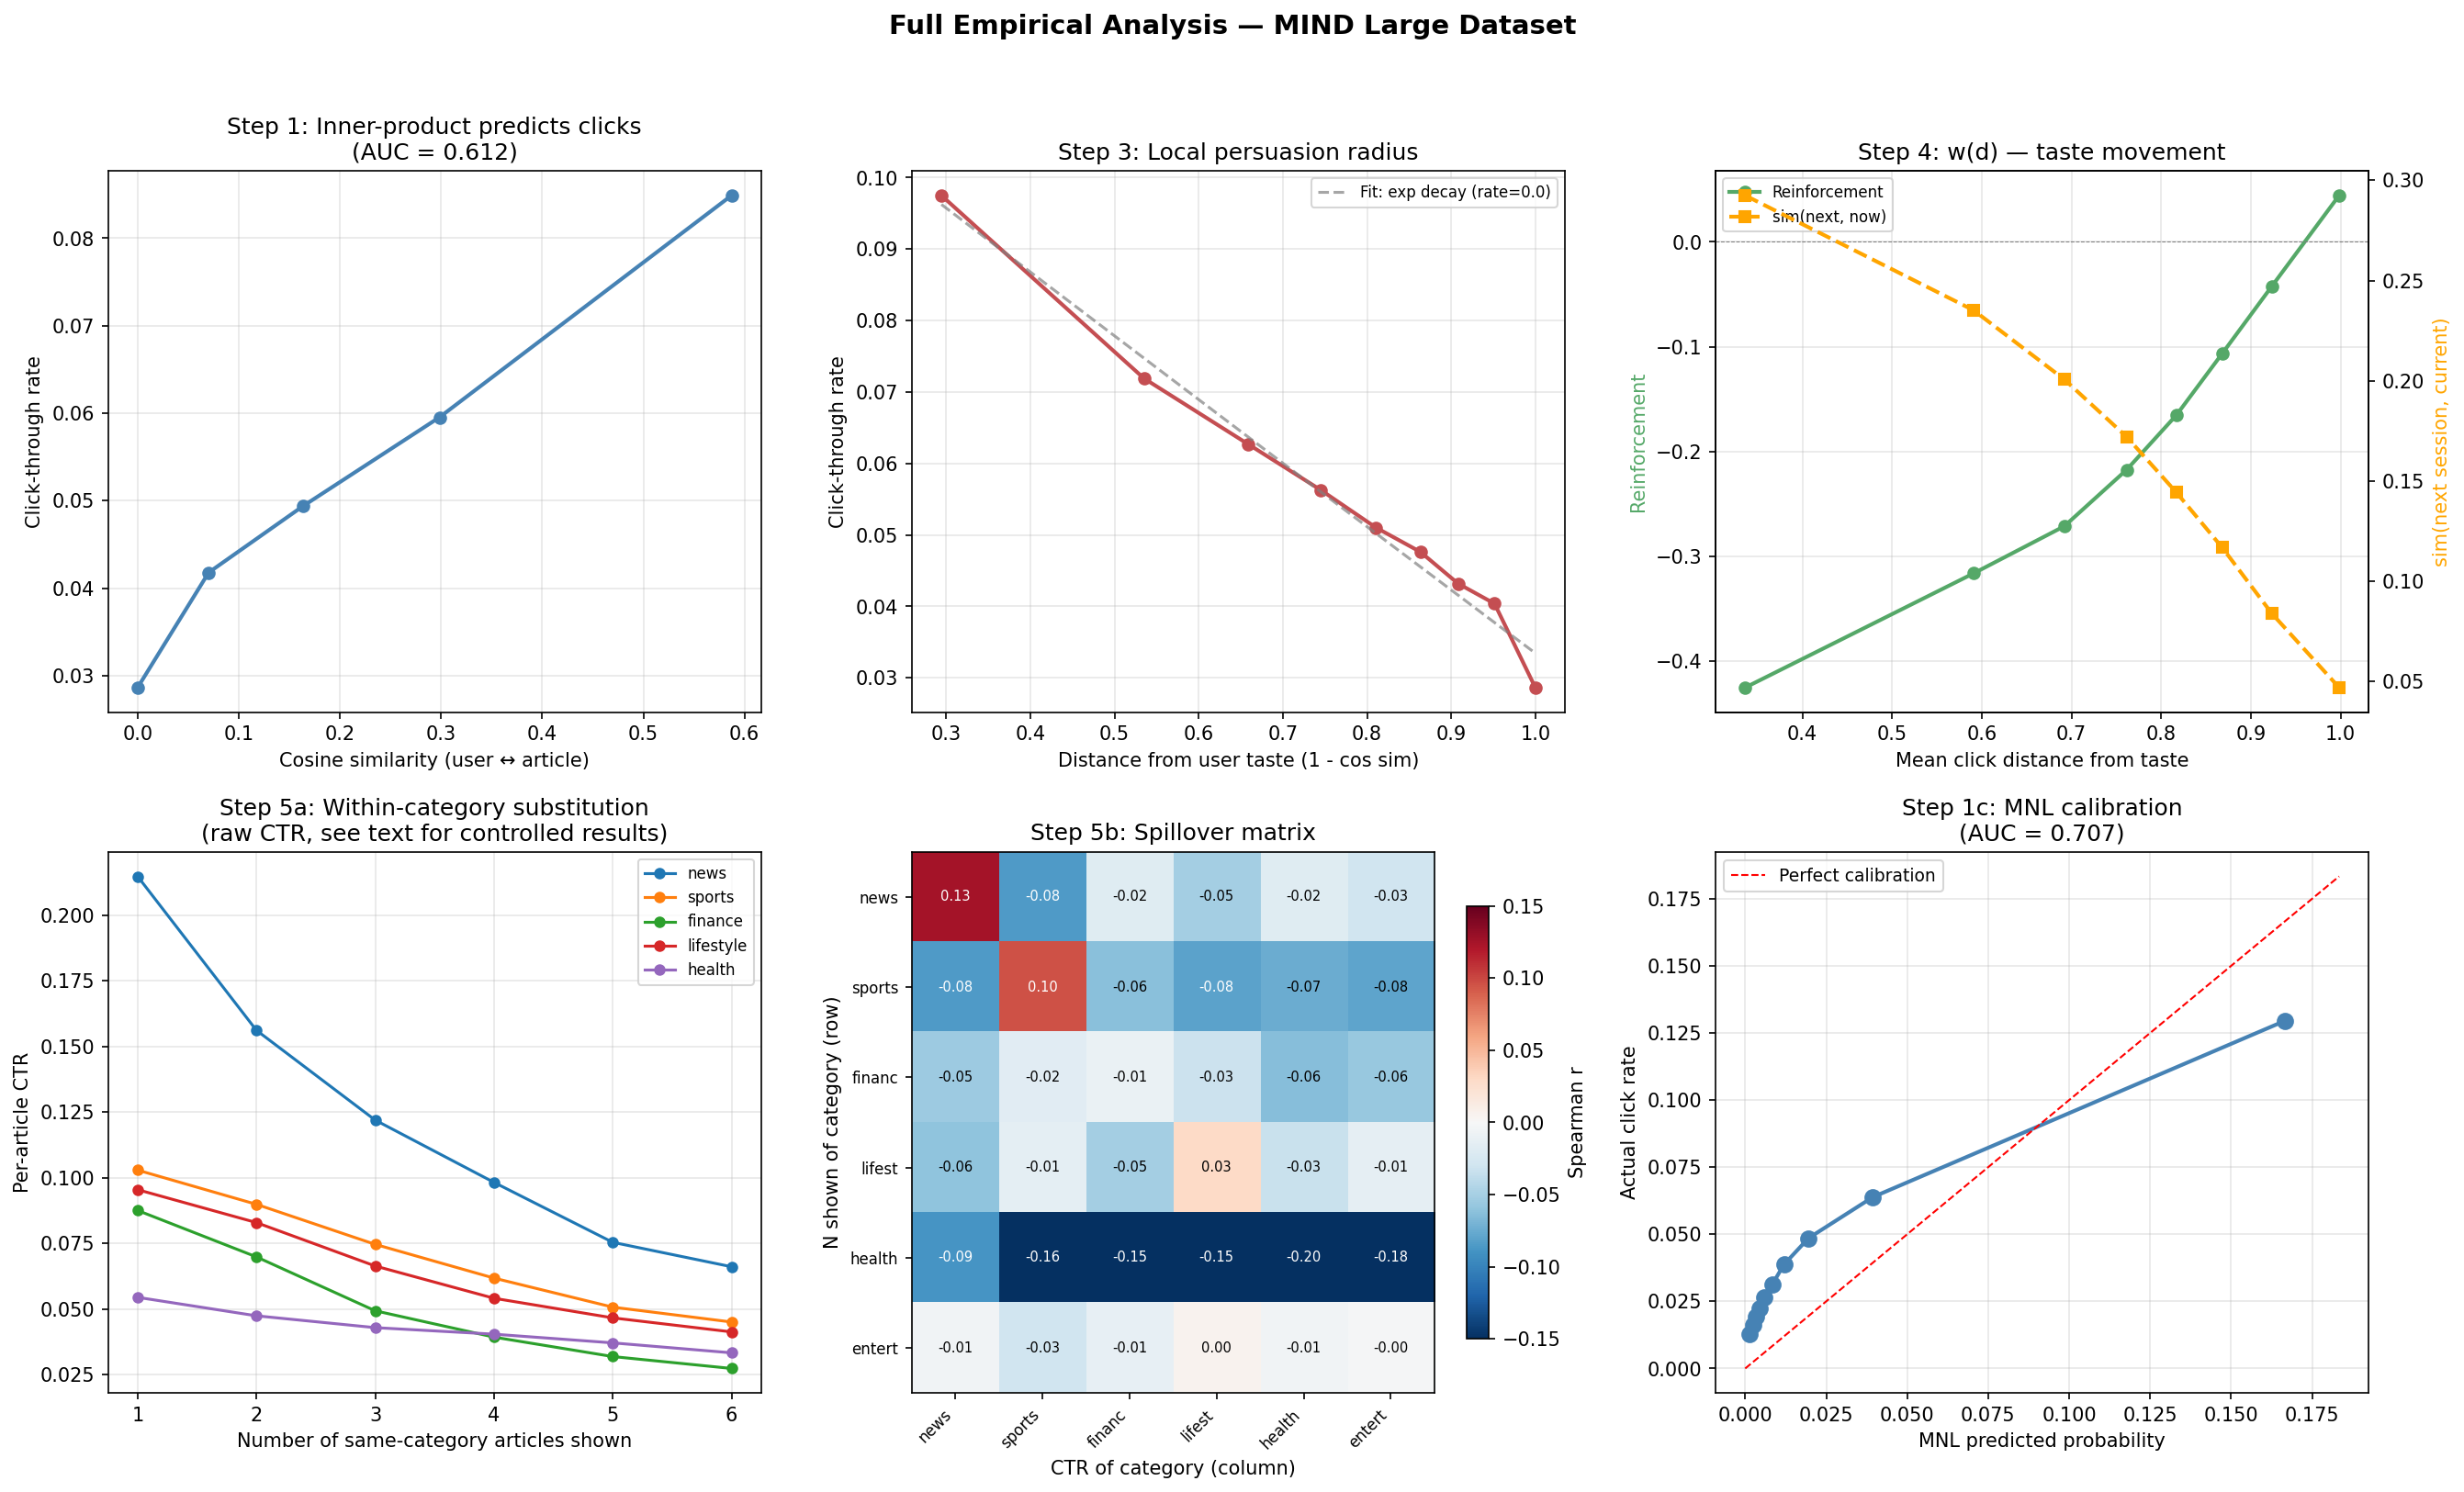
\includegraphics[width=\textwidth]{full_analysis.png}
    \caption{\textbf{(a)}~Cosine similarity vs.\ CTR. \textbf{(b)}~MNL calibration. \textbf{(c)}~CTR decay with distance. \textbf{(d)}~Reinforcement vs.\ click distance. \textbf{(e)}~Within-category substitution. \textbf{(f)}~Cross-category spillover heatmap.}
    \label{fig:full}
\end{figure}
\FloatBarrier

\begin{figure}[ht]
    \centering
    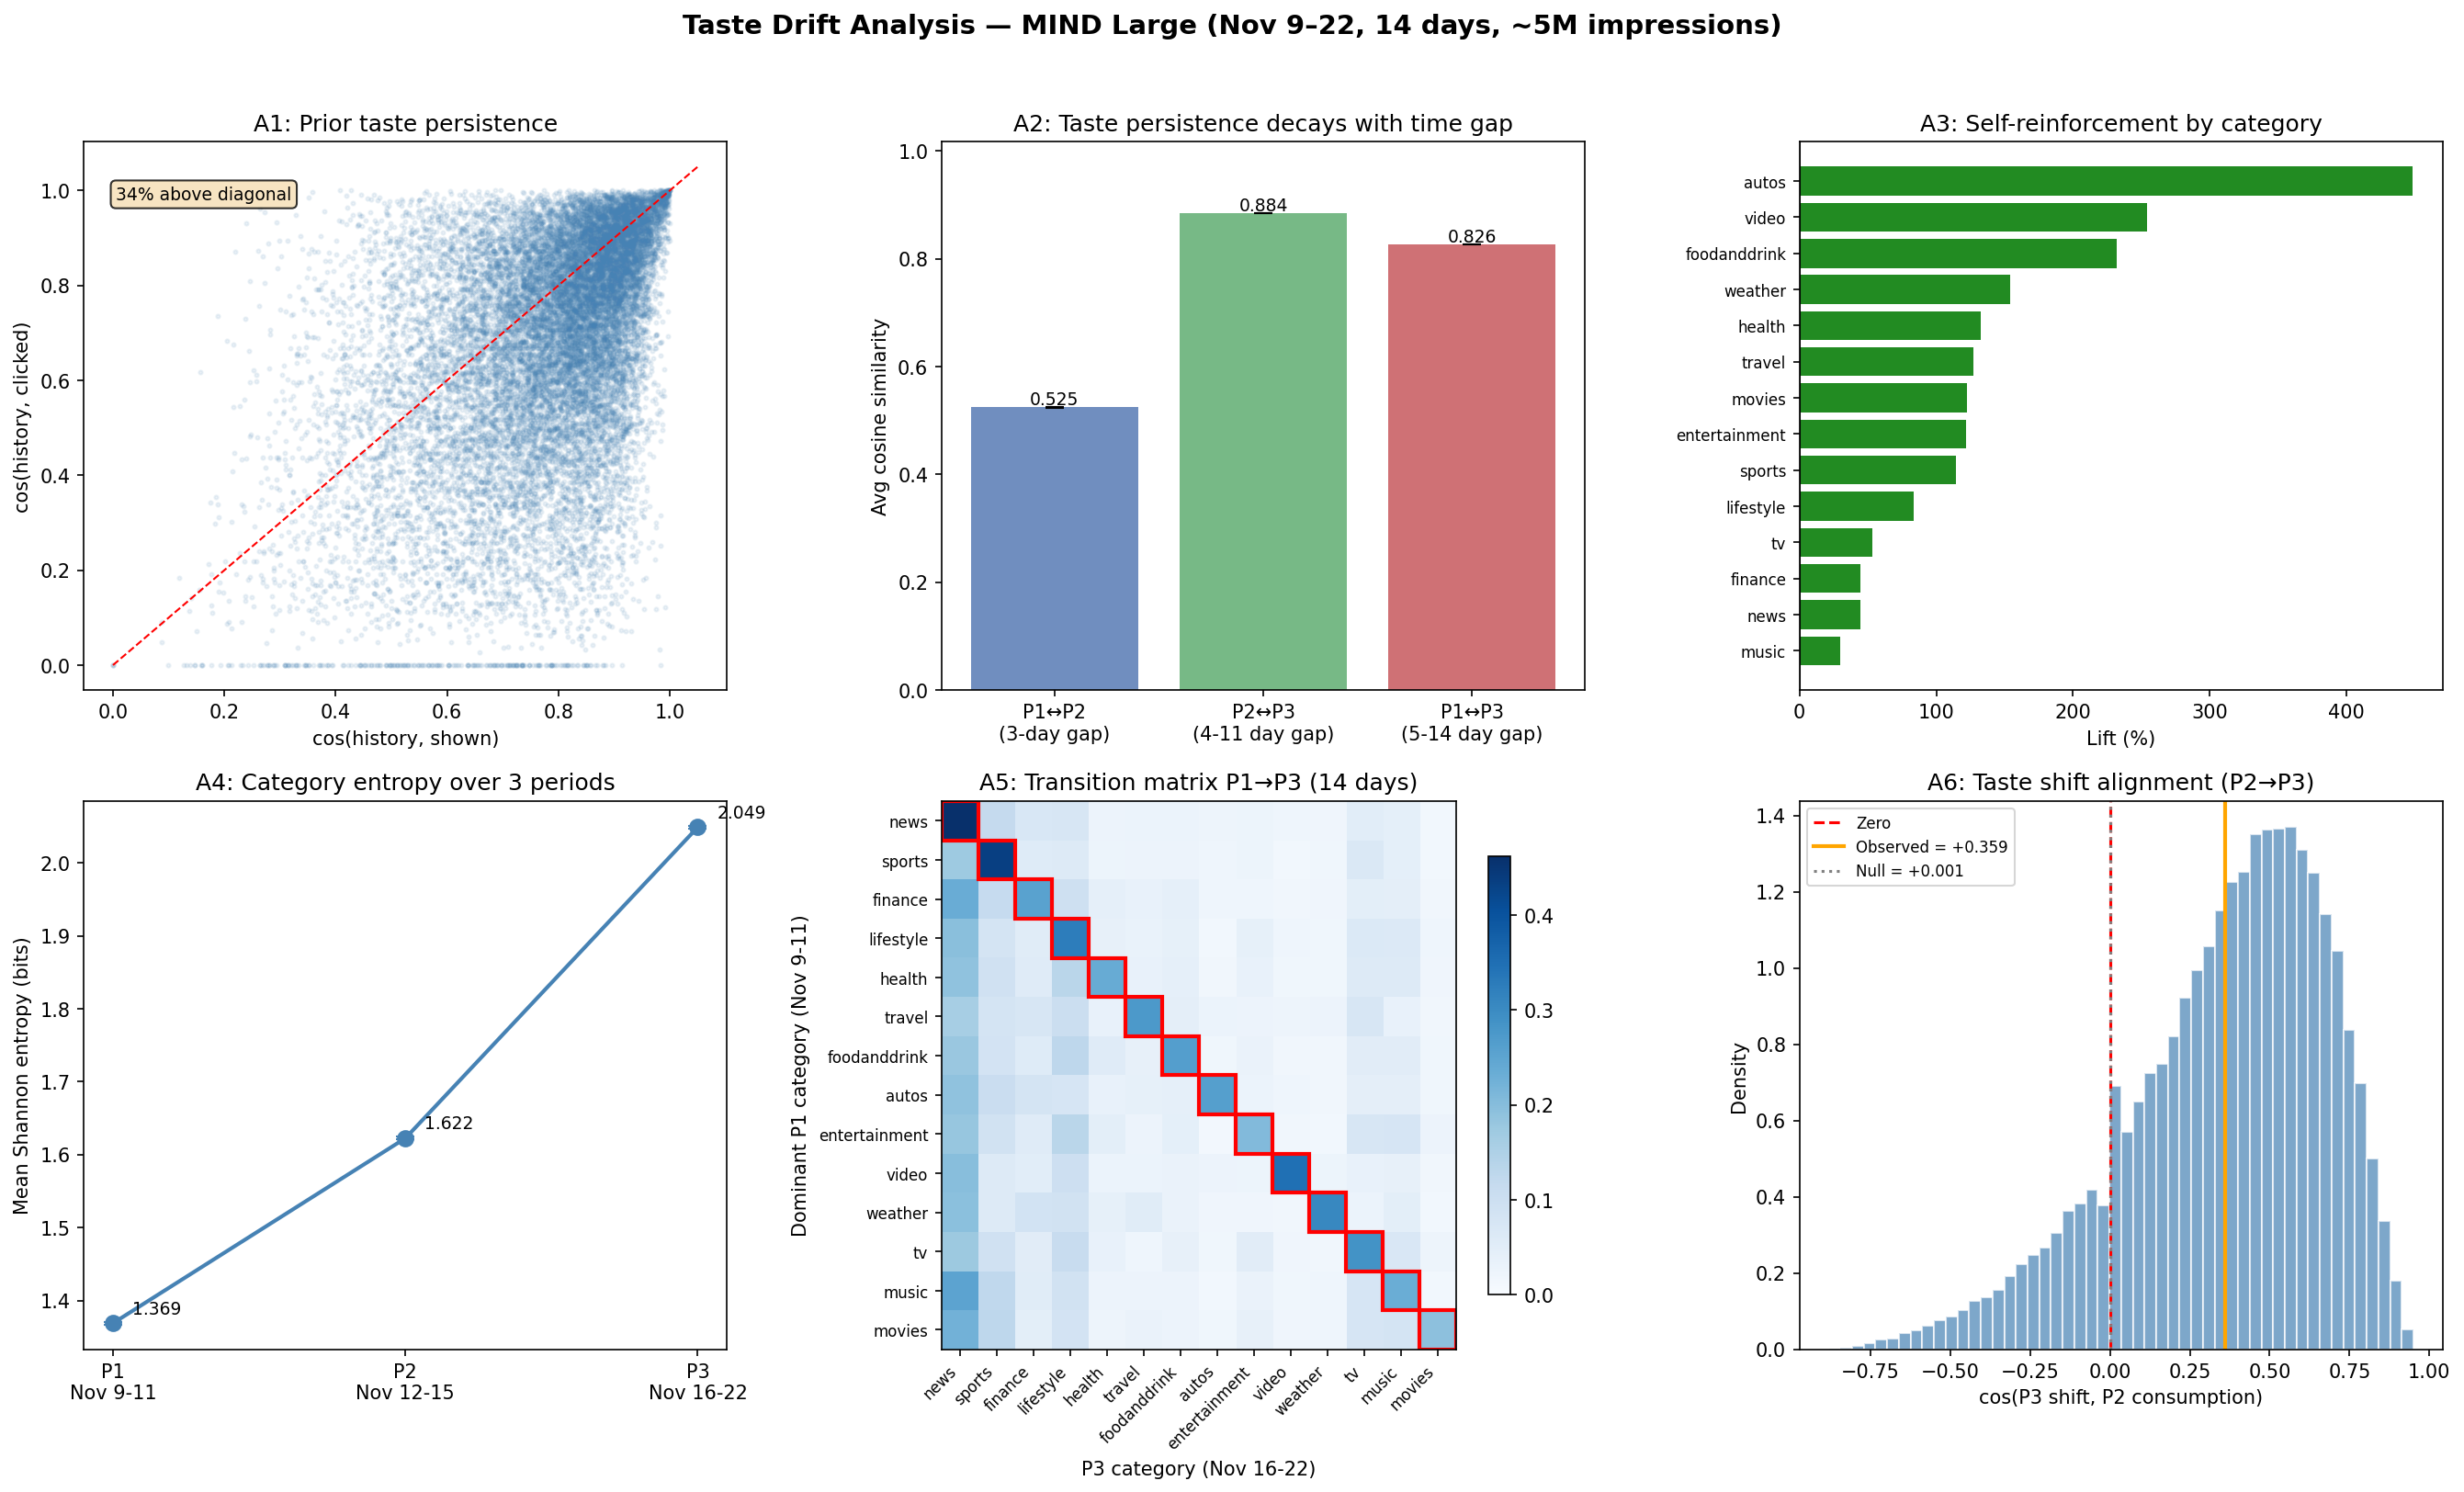
\includegraphics[width=\textwidth]{../output_large/taste_drift_large.png}
    \caption{Taste dynamics. \textbf{(A1)}~Prior taste persistence. \textbf{(A2)}~Similarity decay. \textbf{(A3)}~Self-reinforcement by category. \textbf{(A4)}~Entropy trajectory. \textbf{(A5)}~Transition heatmap. \textbf{(A6)}~Taste shift alignment vs.\ permutation null.}
    \label{fig:drift}
\end{figure}
\FloatBarrier

\begin{figure}[ht]
    \centering
    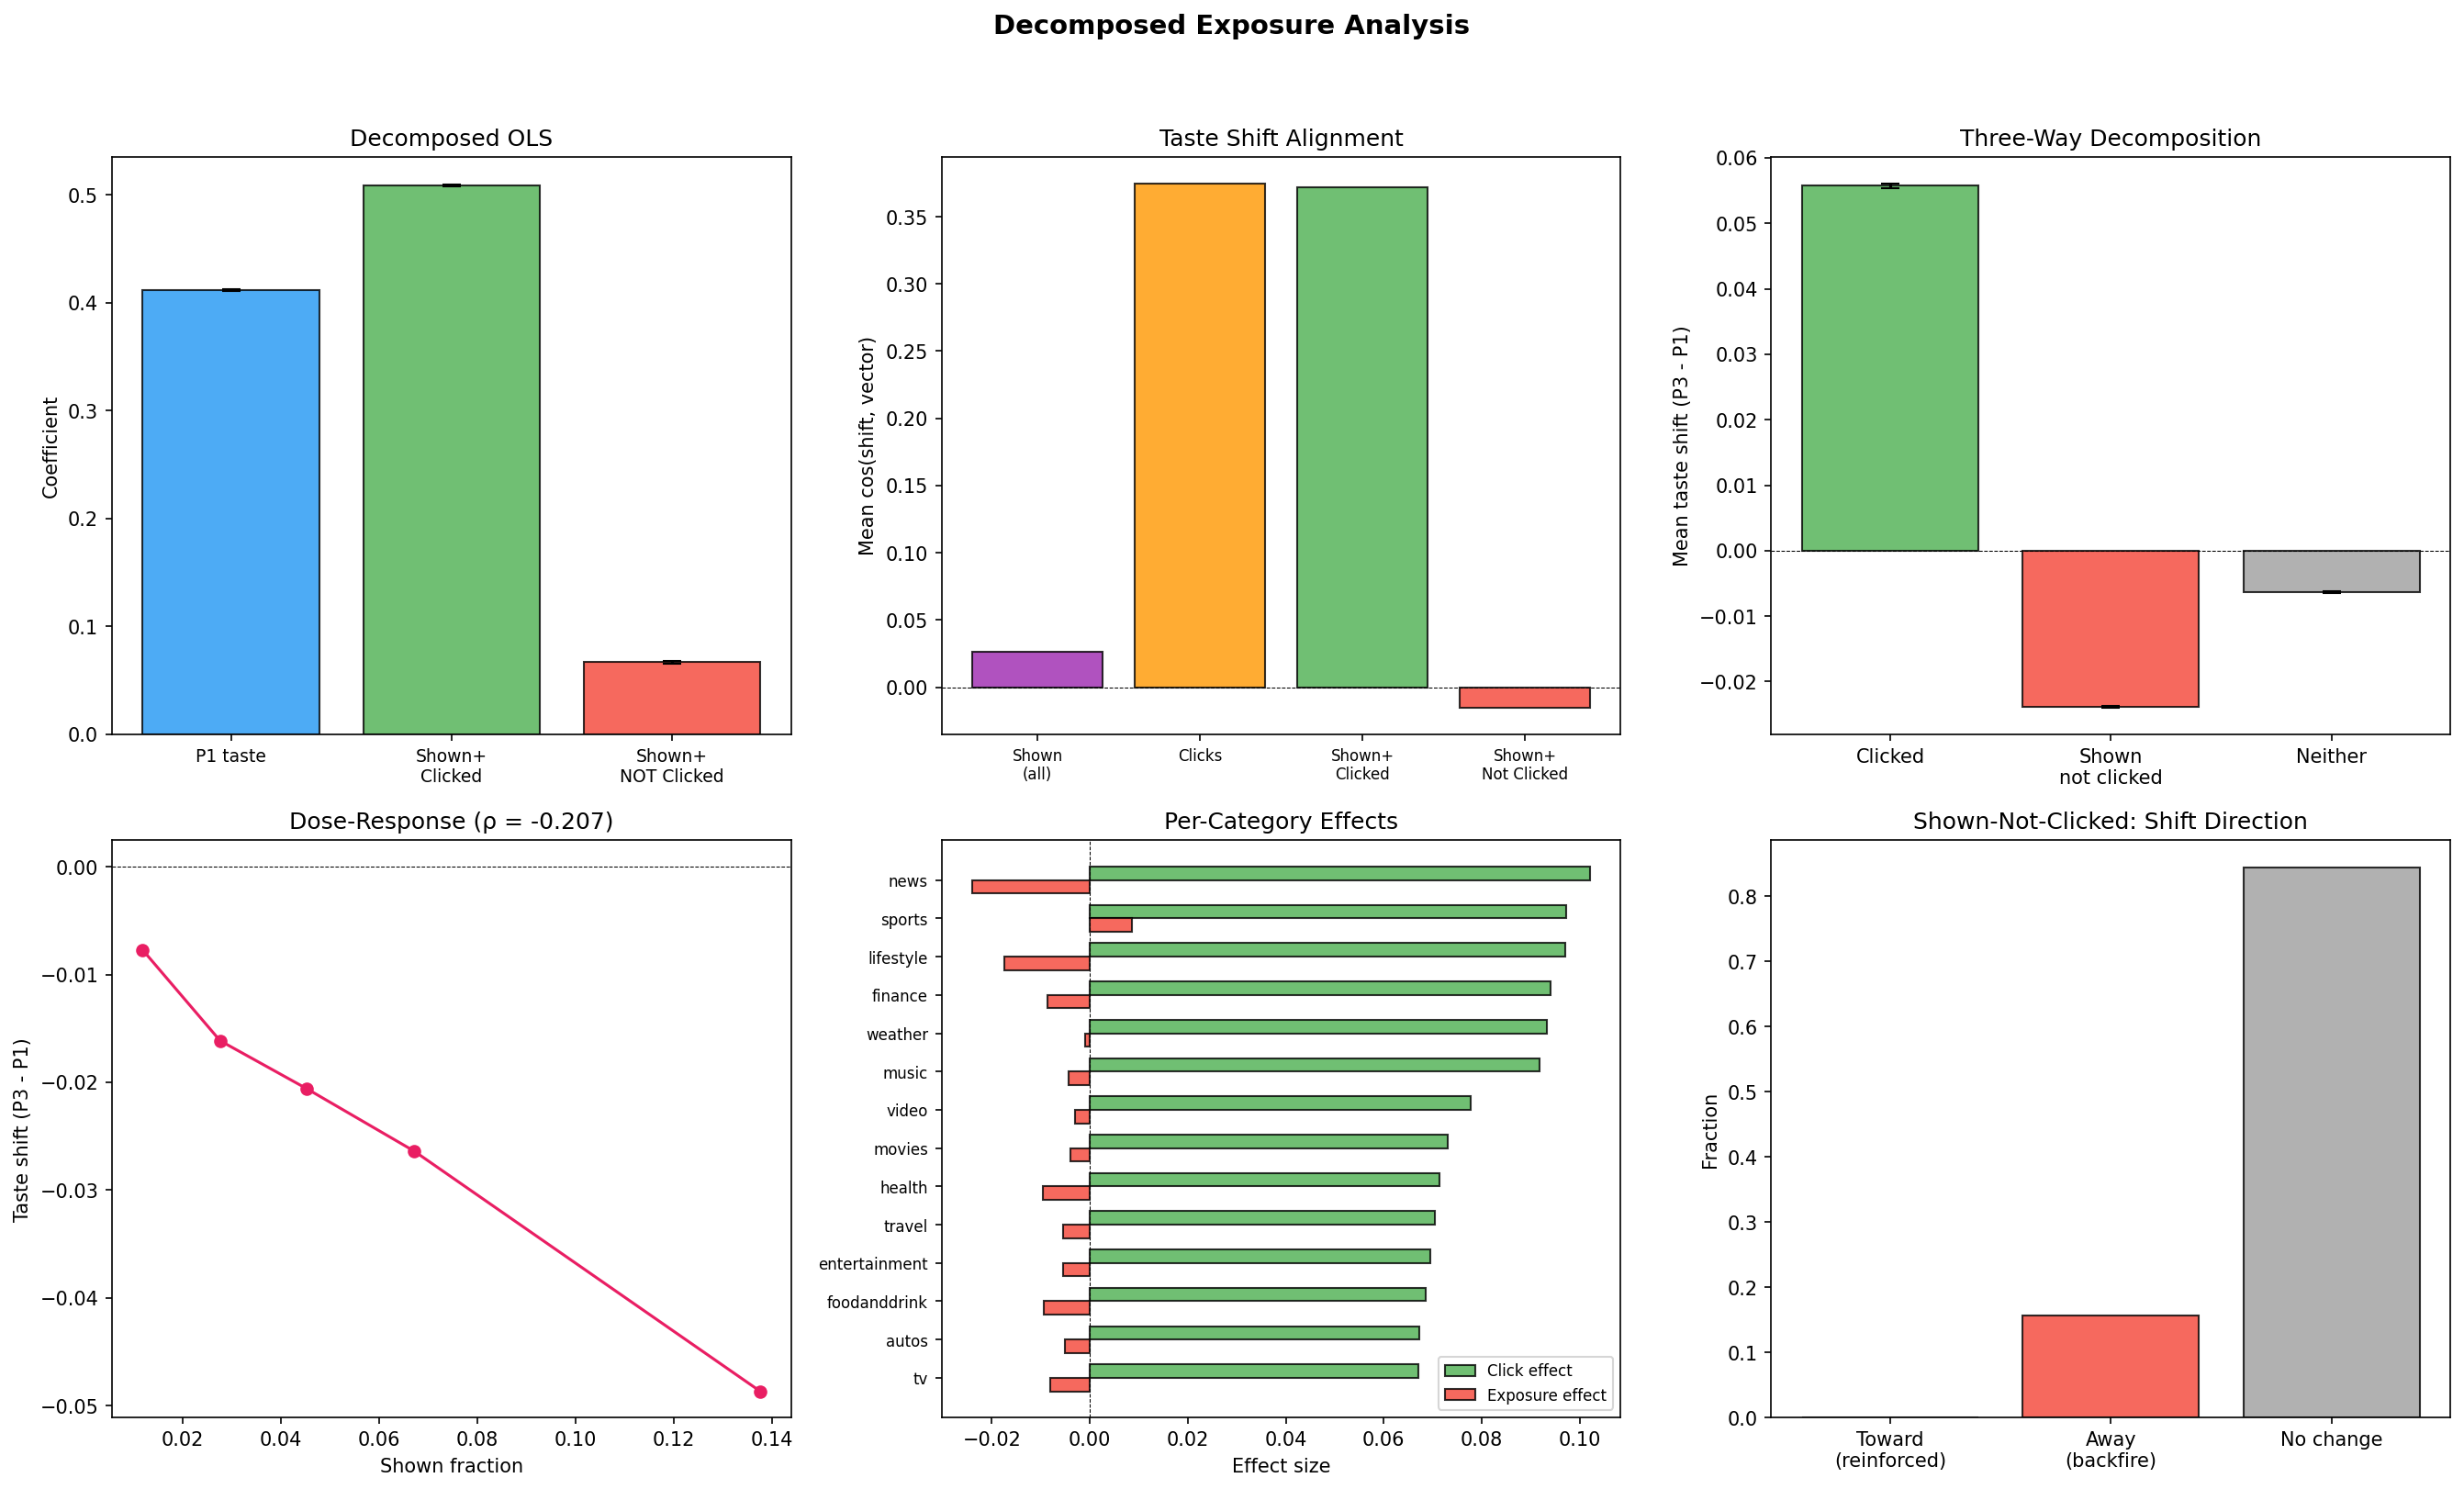
\includegraphics[width=\textwidth]{decomposed_exposure.png}
    \caption{Exposure vs.\ engagement. \textbf{(1)}~Decomposed OLS coefficients. \textbf{(2)}~Four-way cosine alignment. \textbf{(3)}~Three-way taste shift decomposition. \textbf{(4)}~Quintile dose-response. \textbf{(5)}~Per-category click vs.\ exposure effects. \textbf{(6)}~Direction of taste shift for shown-not-clicked pairs.}
    \label{fig:exposure}
\end{figure}
\FloatBarrier

\begin{figure}[ht]
    \centering
    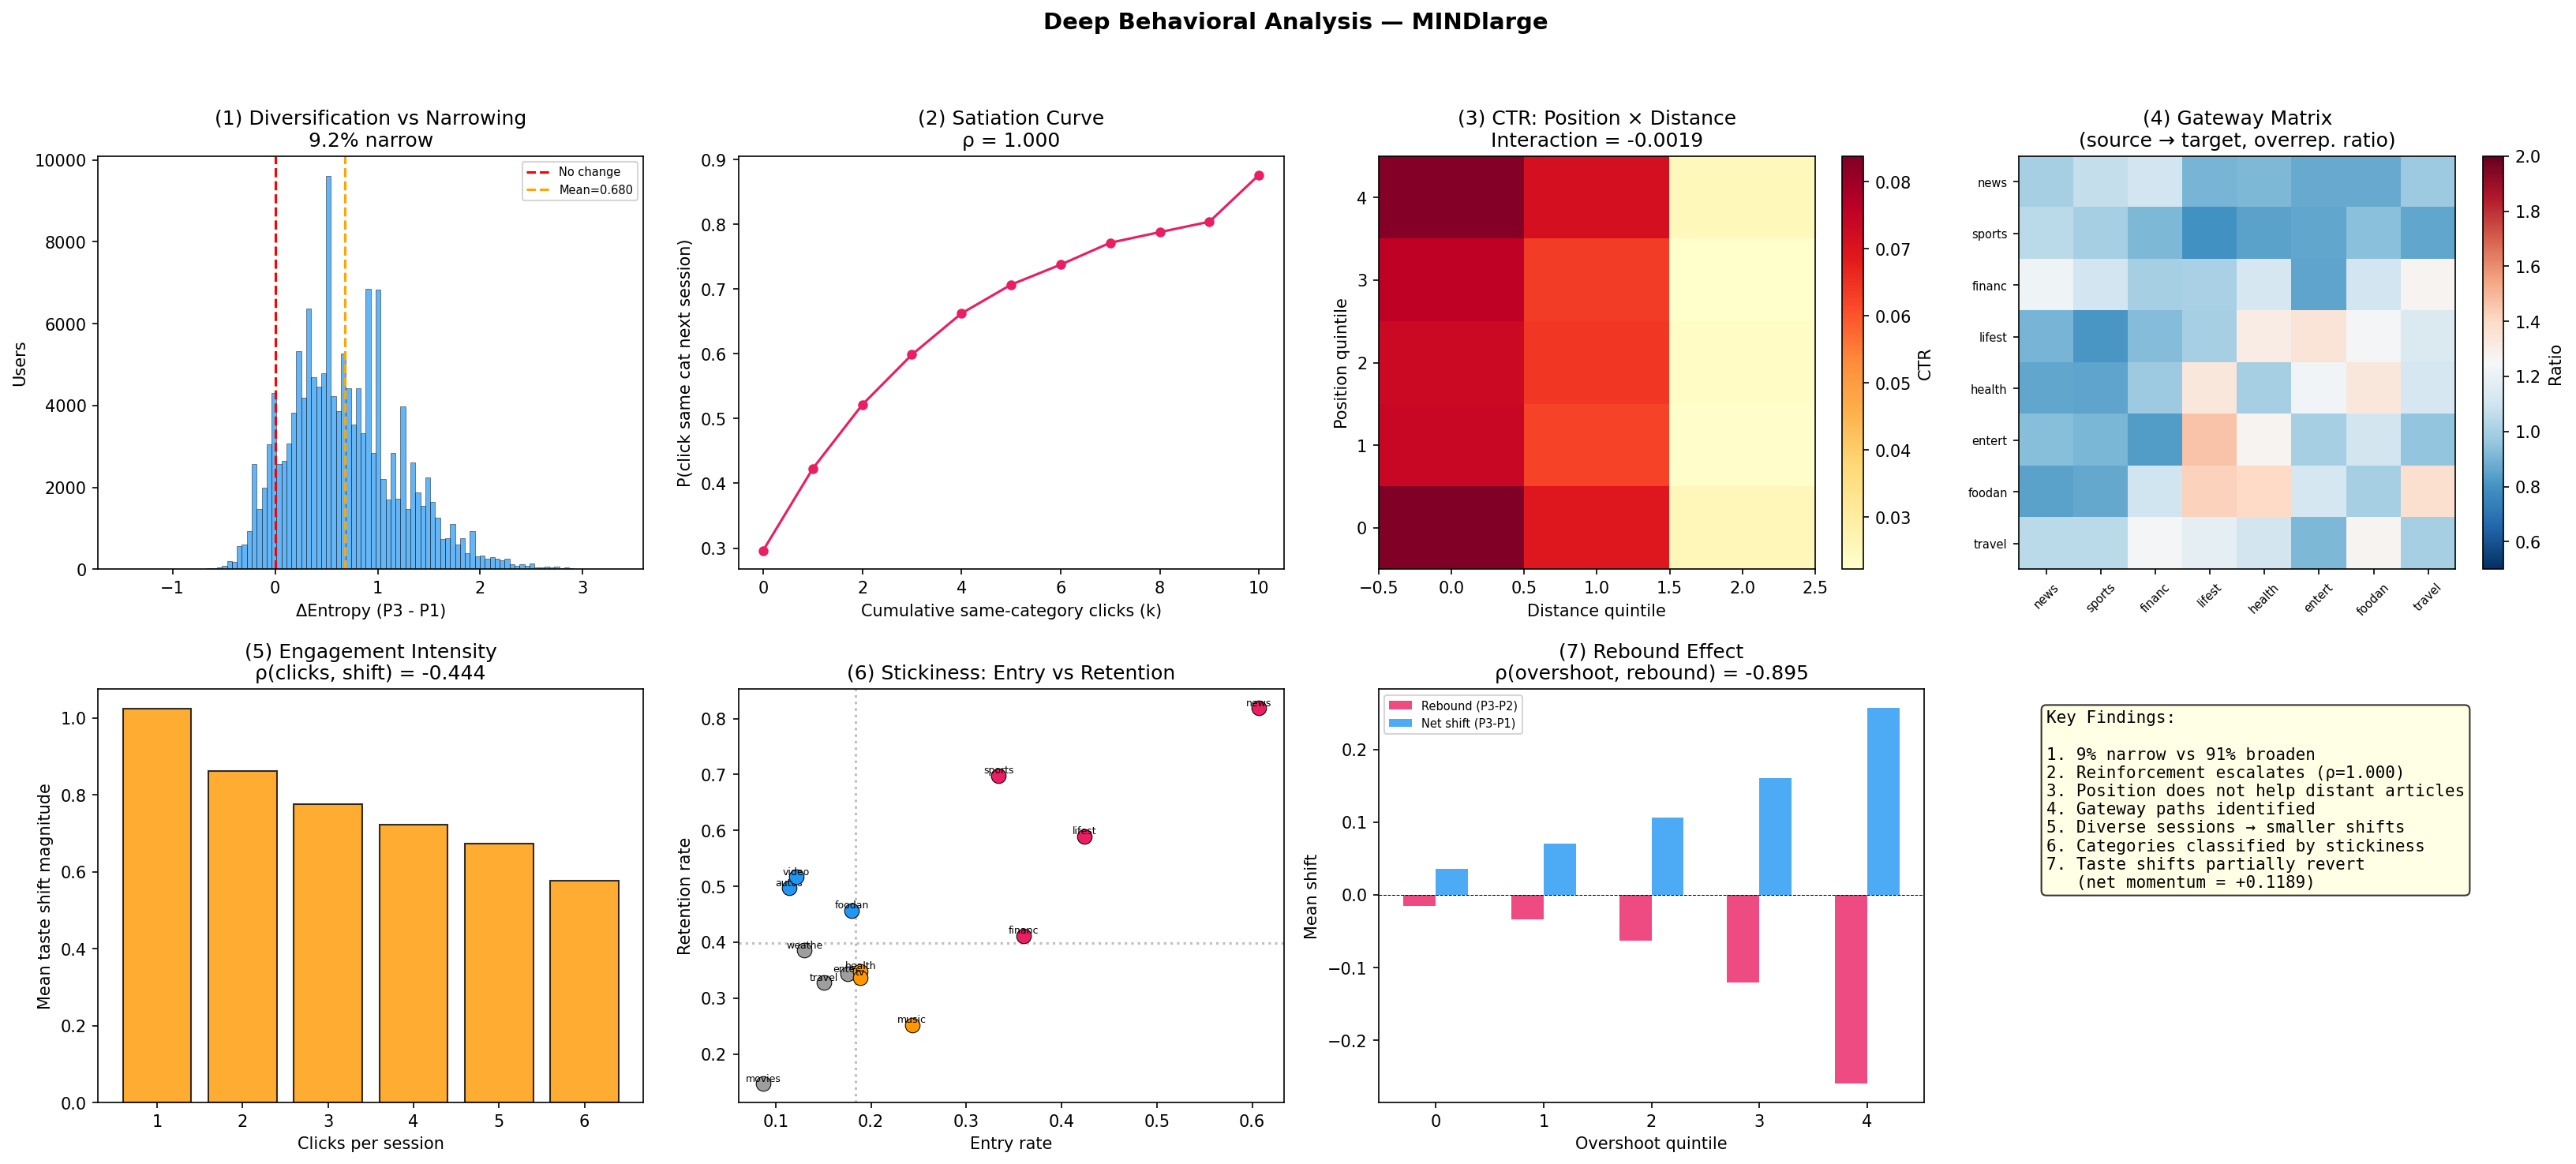
\includegraphics[width=\textwidth]{../output_large/deep_behavioral.png}
    \caption{Fine structure. \textbf{(1)}~Entropy change distribution. \textbf{(2)}~Satiation curves. \textbf{(3)}~Position $\times$ distance heatmap. \textbf{(4)}~Gateway network. \textbf{(5)}~Shift magnitude by session size. \textbf{(6)}~Entry vs.\ retention. \textbf{(7)}~Overshoot vs.\ reversion. \textbf{(8)}~Summary.}
    \label{fig:deep}
\end{figure}
\FloatBarrier


\end{document}
